%%%%%%%%%%%%%%%%%%%%%%%%%%%%%%%%%%%%%%%%%
% The Legrand Orange Book
% LaTeX Template
% Version 1.4 (12/4/14)
%
% This template has been downloaded from:
% http://www.LaTeXTemplates.com
%
% Original author:
% Mathias Legrand (legrand.mathias@gmail.com)
%
% License:
% CC BY-NC-SA 3.0 (http://creativecommons.org/licenses/by-nc-sa/3.0/)
%
% Compiling this template:
% This template uses biber for its bibliography and makeindex for its index.
% When you first open the template, compile it from the command line with the 
% commands below to make sure your LaTeX distribution is configured correctly:
%
% 1) pdflatex main
% 2) makeindex main.idx -s StyleInd.ist
% 3) biber main
% 4) pdflatex main x 2
%
% After this, when you wish to update the bibliography/index use the appropriate
% command above and make sure to compile with pdflatex several times 
% afterwards to propagate your changes to the document.
%
% This template also uses a number of packages which may need to be
% updated to the newest versions for the template to compile. It is strongly
% recommended you update your LaTeX distribution if you have any
% compilation errors.
%
% Important note:
% Chapter heading images should have a 2:1 width:height ratio,
% e.g. 920px width and 460px height.
%
%%%%%%%%%%%%%%%%%%%%%%%%%%%%%%%%%%%%%%%%%

%----------------------------------------------------------------------------------------
%	PACKAGES AND OTHER DOCUMENT CONFIGURATIONS
%----------------------------------------------------------------------------------------

\documentclass[11pt,fleqn]{scrbook} % Default font size and left-justified equations

\usepackage[top=3cm,bottom=3cm,left=3.2cm,right=3.2cm,headsep=10pt,a4paper]{geometry} % Page margins

\usepackage{xcolor} % Required for specifying colors by name
\definecolor{ocre}{RGB}{243,102,25} % Define the orange color used for highlighting throughout the book

% Font Settings
\usepackage{avant} % Use the Avantgarde font for headings
%\usepackage{times} % Use the Times font for headings
\usepackage{mathptmx} % Use the Adobe Times Roman as the default text font together with math symbols from the Sym­bol, Chancery and Com­puter Modern fonts

\usepackage{microtype} % Slightly tweak font spacing for aesthetics
\usepackage[utf8]{inputenc} % Required for including letters with accents
%\usepackage[T1]{fontenc} % Use 8-bit encoding that has 256 glyphs

% Bibliography
%\usepackage[style=alphabetic,sorting=nyt,sortcites=true,autopunct=true,babel=hyphen,hyperref=true,abbreviate=false,backref=true,backend=biber]{biblatex}
%\addbibresource{bibliography.bib} % BibTeX bibliography file
%\defbibheading{bibempty}{}

% Index
\usepackage{calc} % For simpler calculation - used for spacing the index letter headings correctly
\usepackage{makeidx} % Required to make an index
\makeindex % Tells LaTeX to create the files required for indexing

%----------------------------------------------------------------------------------------

%----------------------------------------------------------------------------------------
%	VARIOUS REQUIRED PACKAGES
%----------------------------------------------------------------------------------------

\usepackage{titlesec} % Allows customization of titles

\usepackage{graphicx} % Required for including pictures
\graphicspath{{Pictures/}} % Specifies the directory where pictures are stored

\usepackage{lipsum} % Inserts dummy text

\usepackage{tikz} % Required for drawing custom shapes

\usepackage[english]{babel} % English language/hyphenation

\usepackage{enumitem} % Customize lists
\setlist{nolistsep} % Reduce spacing between bullet points and numbered lists

\usepackage{booktabs} % Required for nicer horizontal rules in tables

\usepackage{eso-pic} % Required for specifying an image background in the title page

%----------------------------------------------------------------------------------------
%	MAIN TABLE OF CONTENTS
%----------------------------------------------------------------------------------------

\usepackage{titletoc} % Required for manipulating the table of contents

\contentsmargin{0cm} % Removes the default margin
% Chapter text styling
\titlecontents{chapter}[1.25cm] % Indentation
{\addvspace{15pt}\large\sffamily\bfseries} % Spacing and font options for chapters
{\color{ocre!60}\contentslabel[\Large\thecontentslabel]{1.25cm}\color{ocre}} % Chapter number
{}  
{\color{ocre!60}\normalsize\sffamily\bfseries\;\titlerule*[.5pc]{.}\;\thecontentspage} % Page number
% Section text styling
\titlecontents{section}[1.25cm] % Indentation
{\addvspace{5pt}\sffamily\bfseries} % Spacing and font options for sections
{\contentslabel[\thecontentslabel]{1.25cm}} % Section number
{}
{\sffamily\hfill\color{black}\thecontentspage} % Page number
[]
% Subsection text styling
\titlecontents{subsection}[1.25cm] % Indentation
{\addvspace{1pt}\sffamily\small} % Spacing and font options for subsections
{\contentslabel[\thecontentslabel]{1.25cm}} % Subsection number
{}
{\sffamily\;\titlerule*[.5pc]{.}\;\thecontentspage} % Page number
[] 

%----------------------------------------------------------------------------------------
%	MINI TABLE OF CONTENTS IN CHAPTER HEADS
%----------------------------------------------------------------------------------------

% Section text styling
\titlecontents{lsection}[0em] % Indendating
{\footnotesize\sffamily} % Font settings
{}
{}
{}

% Subsection text styling
\titlecontents{lsubsection}[.5em] % Indentation
{\normalfont\footnotesize\sffamily} % Font settings
{}
{}
{}
 
%----------------------------------------------------------------------------------------
%	PAGE HEADERS
%----------------------------------------------------------------------------------------

\usepackage{fancyhdr} % Required for header and footer configuration

\pagestyle{fancy}
\renewcommand{\chaptermark}[1]{\markboth{\sffamily\normalsize\bfseries\chaptername\ \thechapter.\ #1}{}} % Chapter text font settings
\renewcommand{\sectionmark}[1]{\markright{\sffamily\normalsize\thesection\hspace{5pt}#1}{}} % Section text font settings
\fancyhf{} \fancyhead[LE,RO]{\sffamily\normalsize\thepage} % Font setting for the page number in the header
\fancyhead[LO]{\rightmark} % Print the nearest section name on the left side of odd pages
\fancyhead[RE]{\leftmark} % Print the current chapter name on the right side of even pages
\renewcommand{\headrulewidth}{0.5pt} % Width of the rule under the header
\addtolength{\headheight}{2.5pt} % Increase the spacing around the header slightly
\renewcommand{\footrulewidth}{0pt} % Removes the rule in the footer
\fancypagestyle{plain}{\fancyhead{}\renewcommand{\headrulewidth}{0pt}} % Style for when a plain pagestyle is specified

% Removes the header from odd empty pages at the end of chapters
\makeatletter
\renewcommand{\cleardoublepage}{
\clearpage\ifodd\c@page\else
\hbox{}
\vspace*{\fill}
\thispagestyle{empty}
\newpage
\fi}

%----------------------------------------------------------------------------------------
%	THEOREM STYLES
%----------------------------------------------------------------------------------------

\usepackage{amsmath,amsfonts,amssymb,amsthm} % For math equations, theorems, symbols, etc

\newcommand{\intoo}[2]{\mathopen{]}#1\,;#2\mathclose{[}}
\newcommand{\ud}{\mathop{\mathrm{{}d}}\mathopen{}}
\newcommand{\intff}[2]{\mathopen{[}#1\,;#2\mathclose{]}}
\newtheorem{notation}{Notation}[chapter]

%%%%%%%%%%%%%%%%%%%%%%%%%%%%%%%%%%%%%%%%%%%%%%%%%%%%%%%%%%%%%%%%%%%%%%%%%%%
%%%%%%%%%%%%%%%%%%%% dedicated to boxed/framed environements %%%%%%%%%%%%%%
%%%%%%%%%%%%%%%%%%%%%%%%%%%%%%%%%%%%%%%%%%%%%%%%%%%%%%%%%%%%%%%%%%%%%%%%%%%
\newtheoremstyle{ocrenumbox}% % Theorem style name
{0pt}% Space above
{0pt}% Space below
{\normalfont}% % Body font
{}% Indent amount
{\small\bf\sffamily\color{ocre}}% % Theorem head font
{\;}% Punctuation after theorem head
{0.25em}% Space after theorem head
{\small\sffamily\color{ocre}\thmname{#1}\nobreakspace\thmnumber{\@ifnotempty{#1}{}\@upn{#2}}% Theorem text (e.g. Theorem 2.1)
\thmnote{\nobreakspace\the\thm@notefont\sffamily\bfseries\color{black}---\nobreakspace#3.}} % Optional theorem note
\renewcommand{\qedsymbol}{$\blacksquare$}% Optional qed square

\newtheoremstyle{blacknumex}% Theorem style name
{5pt}% Space above
{5pt}% Space below
{\normalfont}% Body font
{} % Indent amount
{\small\bf\sffamily}% Theorem head font
{\;}% Punctuation after theorem head
{0.25em}% Space after theorem head
{\small\sffamily{\tiny\ensuremath{\blacksquare}}\nobreakspace\thmname{#1}\nobreakspace\thmnumber{\@ifnotempty{#1}{}\@upn{#2}}% Theorem text (e.g. Theorem 2.1)
\thmnote{\nobreakspace\the\thm@notefont\sffamily\bfseries---\nobreakspace#3.}}% Optional theorem note

\newtheoremstyle{blacknumbox} % Theorem style name
{0pt}% Space above
{0pt}% Space below
{\normalfont}% Body font
{}% Indent amount
{\small\bf\sffamily}% Theorem head font
{\;}% Punctuation after theorem head
{0.25em}% Space after theorem head
{\small\sffamily\thmname{#1}\nobreakspace\thmnumber{\@ifnotempty{#1}{}\@upn{#2}}% Theorem text (e.g. Theorem 2.1)
\thmnote{\nobreakspace\the\thm@notefont\sffamily\bfseries---\nobreakspace#3.}}% Optional theorem note

%%%%%%%%%%%%%%%%%%%%%%%%%%%%%%%%%%%%%%%%%%%%%%%%%%%%%%%%%%%%%%%%%%%%%%%%%%%
%%%%%%%%%%%%% dedicated to non-boxed/non-framed environements %%%%%%%%%%%%%
%%%%%%%%%%%%%%%%%%%%%%%%%%%%%%%%%%%%%%%%%%%%%%%%%%%%%%%%%%%%%%%%%%%%%%%%%%%
\newtheoremstyle{ocrenum}% % Theorem style name
{5pt}% Space above
{5pt}% Space below
{\normalfont}% % Body font
{}% Indent amount
{\small\bf\sffamily\color{ocre}}% % Theorem head font
{\;}% Punctuation after theorem head
{0.25em}% Space after theorem head
{\small\sffamily\color{ocre}\thmname{#1}\nobreakspace\thmnumber{\@ifnotempty{#1}{}\@upn{#2}}% Theorem text (e.g. Theorem 2.1)
\thmnote{\nobreakspace\the\thm@notefont\sffamily\bfseries\color{black}---\nobreakspace#3.}} % Optional theorem note
\renewcommand{\qedsymbol}{$\blacksquare$}% Optional qed square
\makeatother

% Defines the theorem text style for each type of theorem to one of the three styles above
\newcounter{dummy} 
\numberwithin{dummy}{section}
\theoremstyle{ocrenumbox}
\newtheorem{theoremeT}[dummy]{Theorem}
\newtheorem{problem}{Problem}[chapter]
\newtheorem{exerciseT}{Exercise}[chapter]
\theoremstyle{blacknumex}
\newtheorem{exampleT}{Example}[chapter]
\theoremstyle{blacknumbox}
\newtheorem{vocabulary}{Vocabulary}[chapter]
\newtheorem{definitionT}{Definition}[section]
\newtheorem{corollaryT}[dummy]{Corollary}
\theoremstyle{ocrenum}
\newtheorem{proposition}[dummy]{Proposition}

%----------------------------------------------------------------------------------------
%	DEFINITION OF COLORED BOXES
%----------------------------------------------------------------------------------------

\RequirePackage[framemethod=default]{mdframed} % Required for creating the theorem, definition, exercise and corollary boxes

% Theorem box
\newmdenv[skipabove=7pt,
skipbelow=7pt,
backgroundcolor=black!5,
linecolor=ocre,
innerleftmargin=5pt,
innerrightmargin=5pt,
innertopmargin=5pt,
leftmargin=0cm,
rightmargin=0cm,
innerbottommargin=5pt]{tBox}

% Exercise box	  
\newmdenv[skipabove=7pt,
skipbelow=7pt,
rightline=false,
leftline=true,
topline=false,
bottomline=false,
backgroundcolor=ocre!10,
linecolor=ocre,
innerleftmargin=5pt,
innerrightmargin=5pt,
innertopmargin=5pt,
innerbottommargin=5pt,
leftmargin=0cm,
rightmargin=0cm,
linewidth=4pt]{eBox}	

% Definition box
\newmdenv[skipabove=7pt,
skipbelow=7pt,
rightline=false,
leftline=true,
topline=false,
bottomline=false,
linecolor=ocre,
innerleftmargin=5pt,
innerrightmargin=5pt,
innertopmargin=0pt,
leftmargin=0cm,
rightmargin=0cm,
linewidth=4pt,
innerbottommargin=0pt]{dBox}	

% Corollary box
\newmdenv[skipabove=7pt,
skipbelow=7pt,
rightline=false,
leftline=true,
topline=false,
bottomline=false,
linecolor=gray,
backgroundcolor=black!5,
innerleftmargin=5pt,
innerrightmargin=5pt,
innertopmargin=5pt,
leftmargin=0cm,
rightmargin=0cm,
linewidth=4pt,
innerbottommargin=5pt]{cBox}

% Creates an environment for each type of theorem and assigns it a theorem text style from the "Theorem Styles" section above and a colored box from above
\newenvironment{theorem}{\begin{tBox}\begin{theoremeT}}{\end{theoremeT}\end{tBox}}
\newenvironment{exercise}{\begin{eBox}\begin{exerciseT}}{\hfill{\color{ocre}\tiny\ensuremath{\blacksquare}}\end{exerciseT}\end{eBox}}				  
\newenvironment{definition}{\begin{dBox}\begin{definitionT}}{\end{definitionT}\end{dBox}}	
\newenvironment{example}{\begin{exampleT}}{\hfill{\tiny\ensuremath{\blacksquare}}\end{exampleT}}		
\newenvironment{corollary}{\begin{cBox}\begin{corollaryT}}{\end{corollaryT}\end{cBox}}	

%----------------------------------------------------------------------------------------
%	REMARK ENVIRONMENT
%----------------------------------------------------------------------------------------

\newenvironment{remark}{\par\vspace{10pt}\small % Vertical white space above the remark and smaller font size
\begin{list}{}{
\leftmargin=35pt % Indentation on the left
\rightmargin=25pt}\item\ignorespaces % Indentation on the right
\makebox[-2.5pt]{\begin{tikzpicture}[overlay]
\node[draw=ocre!60,line width=1pt,circle,fill=ocre!25,font=\sffamily\bfseries,inner sep=2pt,outer sep=0pt] at (-15pt,0pt){\textcolor{ocre}{R}};\end{tikzpicture}} % Orange R in a circle
\advance\baselineskip -1pt}{\end{list}\vskip5pt} % Tighter line spacing and white space after remark

%----------------------------------------------------------------------------------------
%	SECTION NUMBERING IN THE MARGIN
%----------------------------------------------------------------------------------------

\makeatletter
\renewcommand{\@seccntformat}[1]{\llap{\textcolor{ocre}{\csname the#1\endcsname}\hspace{1em}}}                    
\renewcommand{\section}{\@startsection{section}{1}{\z@}
{-4ex \@plus -1ex \@minus -.4ex}
{1ex \@plus.2ex }
{\normalfont\large\sffamily\bfseries}}
\renewcommand{\subsection}{\@startsection {subsection}{2}{\z@}
{-3ex \@plus -0.1ex \@minus -.4ex}
{0.5ex \@plus.2ex }
{\normalfont\sffamily\bfseries}}
\renewcommand{\subsubsection}{\@startsection {subsubsection}{3}{\z@}
{-2ex \@plus -0.1ex \@minus -.2ex}
{.2ex \@plus.2ex }
{\normalfont\small\sffamily\bfseries}}                        
\renewcommand\paragraph{\@startsection{paragraph}{4}{\z@}
{-2ex \@plus-.2ex \@minus .2ex}
{.1ex}
{\normalfont\small\sffamily\bfseries}}

%----------------------------------------------------------------------------------------
%	HYPERLINKS IN THE DOCUMENTS
%----------------------------------------------------------------------------------------

% For an unclear reason, the package should be loaded now and not later
\usepackage{hyperref}
\hypersetup{hidelinks,backref=true,pagebackref=true,hyperindex=true,colorlinks=false,breaklinks=true,urlcolor= ocre,bookmarks=true,bookmarksopen=false,pdftitle={Title},pdfauthor={Author}}

%----------------------------------------------------------------------------------------
%	CHAPTER HEADINGS
%----------------------------------------------------------------------------------------

% The set-up below should be (sadly) manually adapted to the overall margin page septup controlled by the geometry package loaded in the main.tex document. It is possible to implement below the dimensions used in the goemetry package (top,bottom,left,right)... TO BE DONE

\newcommand{\thechapterimage}{}
\newcommand{\chapterimage}[1]{\renewcommand{\thechapterimage}{#1}}

% Numbered chapters with mini tableofcontents
\def\thechapter{\arabic{chapter}}
\def\@makechapterhead#1{
\thispagestyle{empty}
{\centering \normalfont\sffamily
\ifnum \c@secnumdepth >\m@ne
\if@mainmatter
\startcontents
\begin{tikzpicture}[remember picture,overlay]
\node at (current page.north west)
{\begin{tikzpicture}[remember picture,overlay]
\node[anchor=north west,inner sep=0pt] at (0,0) {\includegraphics[width=\paperwidth]{\thechapterimage}};
%%%%%%%%%%%%%%%%%%%%%%%%%%%%%%%%%%%%%%%%%%%%%%%%%%%%%%%%%%%%%%%%%%%%%%%%%%%%%%%%%%%%%
% Commenting the 3 lines below removes the small contents box in the chapter heading
\fill[color=ocre!10!white,opacity=.6] (1cm,0) rectangle (8cm,-7cm);
\node[anchor=north west] at (1.1cm,.35cm) {\parbox[t][8cm][t]{6.5cm}{\huge\bfseries\flushleft \printcontents{l}{1}{\setcounter{tocdepth}{2}}}};
\draw[anchor=west] (5cm,-9cm) node [rounded corners=20pt,fill=ocre!10!white,text opacity=1,draw=ocre,draw opacity=1,line width=1.5pt,fill opacity=.6,inner sep=12pt]{\huge\sffamily\bfseries\textcolor{black}{\thechapter. #1\strut\makebox[22cm]{}}};
%%%%%%%%%%%%%%%%%%%%%%%%%%%%%%%%%%%%%%%%%%%%%%%%%%%%%%%%%%%%%%%%%%%%%%%%%%%%%%%%%%%%%
\end{tikzpicture}};
\end{tikzpicture}}
\par\vspace*{230\p@}
\fi
\fi}

% Unnumbered chapters without mini tableofcontents (could be added though) 
\def\@makeschapterhead#1{
\thispagestyle{empty}
{\centering \normalfont\sffamily
\ifnum \c@secnumdepth >\m@ne
\if@mainmatter
\begin{tikzpicture}[remember picture,overlay]
\node at (current page.north west)
{\begin{tikzpicture}[remember picture,overlay]
\node[anchor=north west,inner sep=0pt] at (0,0) {\includegraphics[width=\paperwidth]{\thechapterimage}};
\draw[anchor=west] (5cm,-9cm) node [rounded corners=20pt,fill=ocre!10!white,fill opacity=.6,inner sep=12pt,text opacity=1,draw=ocre,draw opacity=1,line width=1.5pt]{\huge\sffamily\bfseries\textcolor{black}{#1\strut\makebox[22cm]{}}};
\end{tikzpicture}};
\end{tikzpicture}}
\par\vspace*{230\p@}
\fi
\fi
}
\makeatother % Insert the commands.tex file which contains the majority of the structure behind the template

%----------------------------------------------------------------------------------------
% Added for dschungelbuch

\usepackage{eurosym}
\usepackage{hyperref}
\usepackage{url}
\usepackage{csquotes}
\setlength{\parindent}{0pt}
\usepackage{pdfpages}

\begin{document}

%----------------------------------------------------------------------------------------
%	TITLE PAGE
%----------------------------------------------------------------------------------------

\begingroup
\thispagestyle{empty}
\AddToShipoutPicture*{\put(6,5){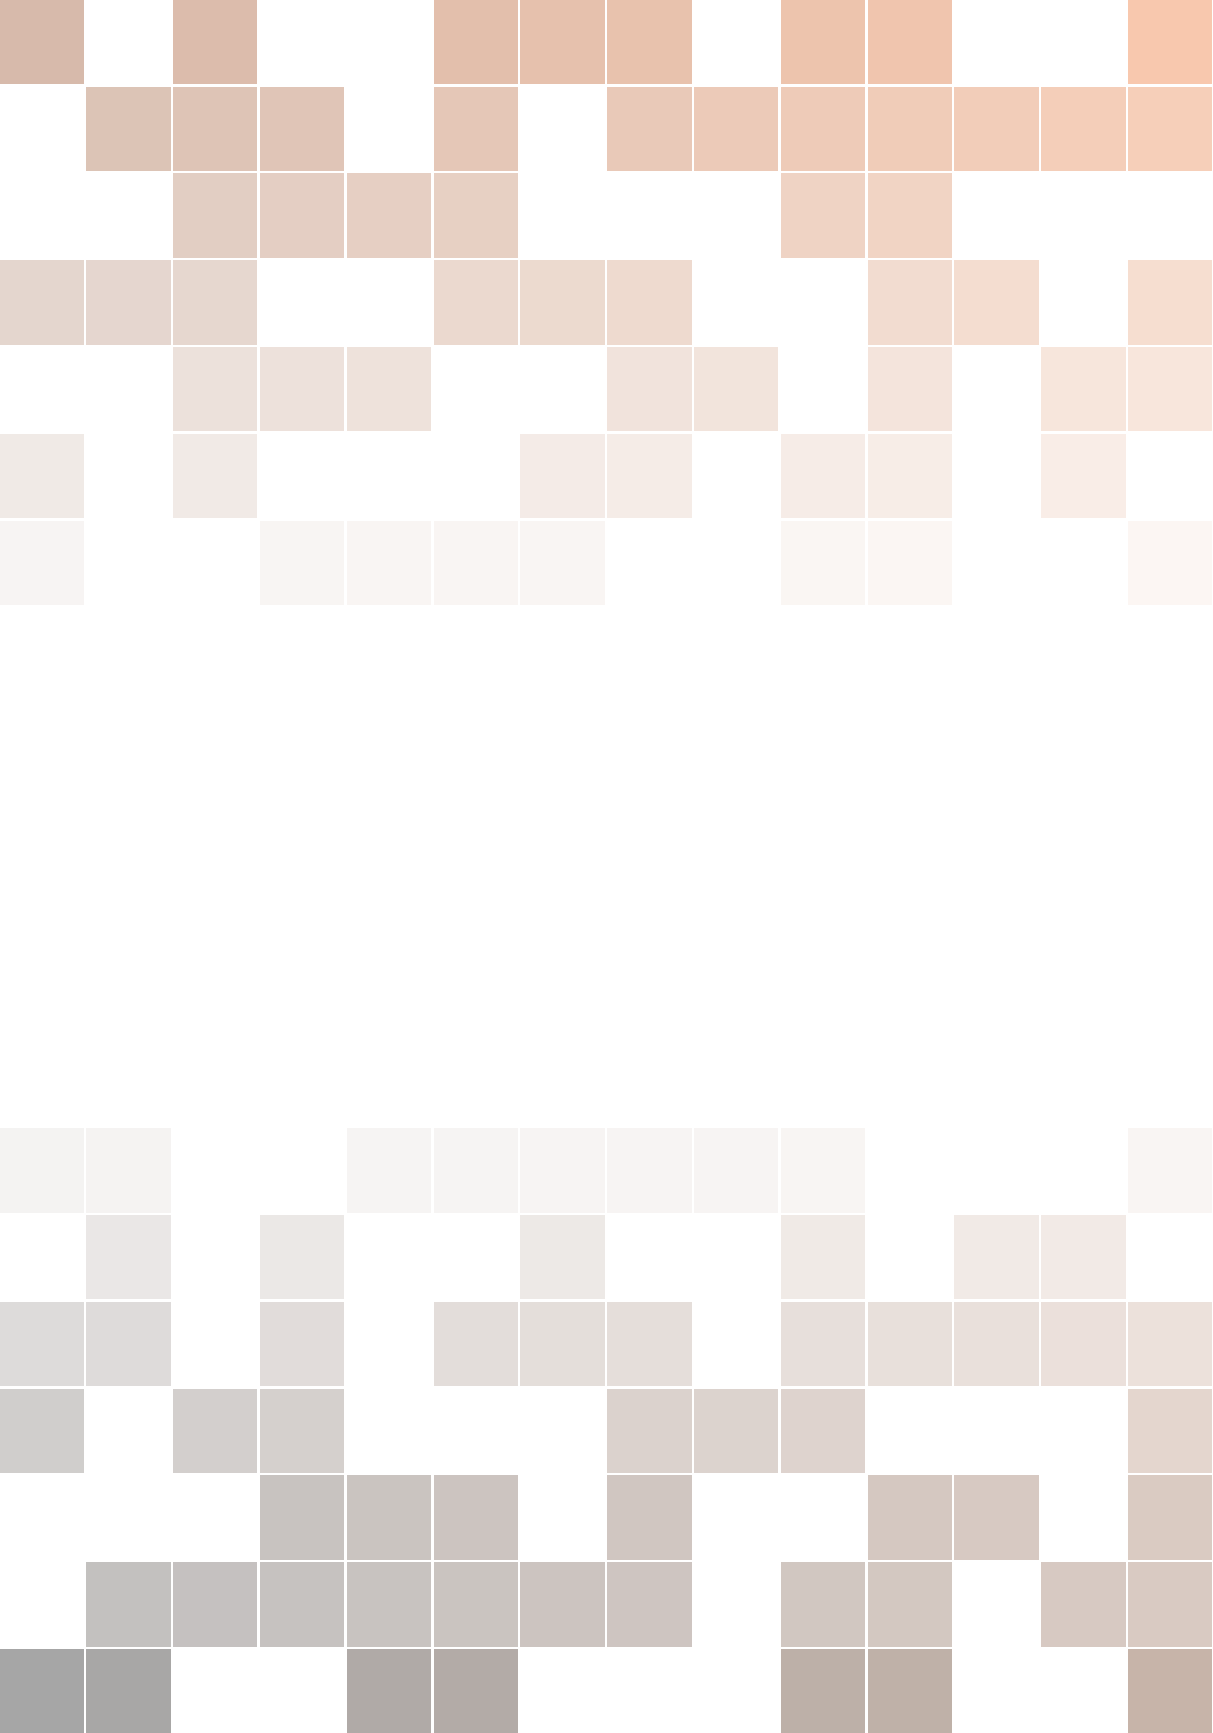
\includegraphics[scale=1]{background}}} % Image background
\centering
\vspace*{9cm}
\par\normalfont\fontsize{35}{35}\sffamily\selectfont
Dschungelbuch Siegen\\ {\LARGE Information für Menschen mit wenig Geld in und um Siegen}\par % Book title
\vspace*{1cm}
{\Huge Klaus Reifenrath}\par % Author name
\endgroup

%----------------------------------------------------------------------------------------
%	COPYRIGHT PAGE
%----------------------------------------------------------------------------------------

\newpage
~\vfill
\thispagestyle{empty}

\noindent Kein Copyright / no \copyright. Kopieren und Verteilen ausdrücklich erlaubt.\\ % Copyright notice

\noindent \textsc{Published by Klaus Reifenrath}\\ % Publisher

\noindent \textsc{www.krwe.de, klaus@krwe.de}\\ % URL

%\noindent Licensed under the Creative Commons Attribution-NonCommercial 3.0 Unported License (the ``License''). You may not use this file except in compliance with the License. You may obtain a copy of the License at \url{http://creativecommons.org/licenses/by-nc/3.0}. Unless required by applicable law or agreed to in writing, software distributed under the License is distributed on an \textsc{``as is'' basis, without warranties or conditions of any kind}, either express or implied. See the License for the specific language governing permissions and limitations under the License.\\ % License information

%\noindent \textit{First printing, March 2013} % Printing/edition date

%----------------------------------------------------------------------------------------
%	TABLE OF CONTENTS
%----------------------------------------------------------------------------------------

\chapterimage{chapter_head_1.pdf} % Table of contents heading image

\pagestyle{empty} % No headers

\tableofcontents % Print the table of contents itself

\cleardoublepage % Forces the first chapter to start on an odd page so it's on the right

\pagestyle{fancy} % Print headers again

%----------------------------------------------------------------------------------------
%	Vorwort
%----------------------------------------------------------------------------------------

\section{Vorwort von Klaus Reifenrath}

Informationen für Menschen in und um Siegen mit  wenig oder keinem Einkommen. Die Idee zum „Dschungelbuch Siegen“ ist mit Freunden und Betroffenen entstanden. Wir haben diese Informationen zusammengestellt und sie unter dem Namen \enquote{Dschungelbuch Siegen} im Internet veröffentlicht. Zu finden über Google \enquote{Dschungelbuch Siegen} oder unter \href{http://www.krwe.de}{ www.krwe.de}. Dort können Sie das \enquote{Dschungelbuch Siegen} kostenlos herunterladen, lesen oder ausdrucken und gerne an Menschen, die es interessiert, weitergeben. Es besteht kein Copyright und kein kommerzielles Interesse! Bitte weiterreichen. Es soll einfach nur eine Hilfe im Dschungel der Stadt darstellen. Wir suchen nach weiteren sozialen Einrichtungen in Siegen und Umgebung, damit wir das \enquote{Dschungelbuch Siegen} erweitern können. Senden Sie uns bitte per Mail eine Nachricht an \href{mailto:klaus@krwe.de}{klaus@krwe}, wenn Sie im \enquote{Dschungelbuch Siegen} etwas lesen, das sich geändert hat.

\section{Vorwort von nanooq}

Das Layout des Dschungelbuchs basiert \enquote{The Legrand Orange Book} von Mathias Legrand \href{mailto:legrand.mathias@gmail.com}{legrand.mathias@gmail.com} und steht unter \enquote{CC BY-NC-SA 3.0}. Das Dschungelbuch kam durch Uschi Shure über Esteban Shure an mich. Diese Version wird ebenfalls unter CC BY-NC-SA 3.0 im github-repository \href{https://github.com/nanooq/dschungelbuch-siegen}{https://github.com/nanooq/dschungelbuch-siegen} gehostet. Dort wird auch erklärt, wie man Einträge direkt aktualisieren kann. Weitergabe und Mitarbeit erwünscht. Danke an alle Hände und Köpfe, die mitmachen, ihr wisst, wer ihr seid. Viel Spaß beim Lesen und Verteilen!
\chapterimage{chapter_head_2.pdf} % Chapter heading image

%\chapter{Vorlagen}

%------------------------------------------------

\section{Citation}\index{Citation}

This statement requires citation \cite{book_key}; this one is more specific \cite[122]{article_key}.

%------------------------------------------------

\section{Lists}\index{Lists}

Lists are useful to present information in a concise and/or ordered way\footnote{Footnote example...}.

\subsection{Numbered List}\index{Lists!Numbered List}

\begin{enumerate}
\item The first item
\item The second item
\item The third item
\end{enumerate}

\subsection{Bullet Points}\index{Lists!Bullet Points}

\begin{itemize}
\item The first item
\item The second item
\item The third item
\end{itemize}

\subsection{Descriptions and Definitions}\index{Lists!Descriptions and Definitions}

\begin{description}
\item[Name] Description
\item[Word] Definition
\item[Comment] Elaboration
\end{description}

%----------------------------------------------------------------------------------------
%	CHAPTER 2
%----------------------------------------------------------------------------------------

\chapter{In-text Elements}

\section{Theorems}\index{Theorems}

This is an example of theorems.

\subsection{Several equations}\index{Theorems!Several Equations}
This is a theorem consisting of several equations.

\begin{theorem}[Name of the theorem]
In $E=\mathbb{R}^n$ all norms are equivalent. It has the properties:
\begin{align}
& \big| ||\mathbf{x}|| - ||\mathbf{y}|| \big|\leq || \mathbf{x}- \mathbf{y}||\\
&  ||\sum_{i=1}^n\mathbf{x}_i||\leq \sum_{i=1}^n||\mathbf{x}_i||\quad\text{where $n$ is a finite integer}
\end{align}
\end{theorem}

\subsection{Single Line}\index{Theorems!Single Line}
This is a theorem consisting of just one line.

\begin{theorem}
A set $\mathcal{D}(G)$ in dense in $L^2(G)$, $|\cdot|_0$. 
\end{theorem}

%------------------------------------------------

\section{Definitions}\index{Definitions}

This is an example of a definition. A definition could be mathematical or it could define a concept.

\begin{definition}[Definition name]
Given a vector space $E$, a norm on $E$ is an application, denoted $||\cdot||$, $E$ in $\mathbb{R}^+=[0,+\infty[$ such that:
\begin{align}
& ||\mathbf{x}||=0\ \Rightarrow\ \mathbf{x}=\mathbf{0}\\
& ||\lambda \mathbf{x}||=|\lambda|\cdot ||\mathbf{x}||\\
& ||\mathbf{x}+\mathbf{y}||\leq ||\mathbf{x}||+||\mathbf{y}||
\end{align}
\end{definition}

%------------------------------------------------

\section{Notations}\index{Notations}

\begin{notation}
Given an open subset $G$ of $\mathbb{R}^n$, the set of functions $\varphi$ are:
\begin{enumerate}
\item Bounded support $G$;
\item Infinitely differentiable;
\end{enumerate}
a vector space is denoted by $\mathcal{D}(G)$. 
\end{notation}

%------------------------------------------------

\section{Remarks}\index{Remarks}

This is an example of a remark.

\begin{remark}
The concepts presented here are now in conventional employment in mathematics. Vector spaces are taken over the field $\mathbb{K}=\mathbb{R}$, however, established properties are easily extended to $\mathbb{K}=\mathbb{C}$.
\end{remark}

%------------------------------------------------

\section{Corollaries}\index{Corollaries}

This is an example of a corollary.

\begin{corollary}[Corollary name]
The concepts presented here are now in conventional employment in mathematics. Vector spaces are taken over the field $\mathbb{K}=\mathbb{R}$, however, established properties are easily extended to $\mathbb{K}=\mathbb{C}$.
\end{corollary}

%------------------------------------------------

\section{Propositions}\index{Propositions}

This is an example of propositions.

\subsection{Several equations}\index{Propositions!Several Equations}

\begin{proposition}[Proposition name]
It has the properties:
\begin{align}
& \big| ||\mathbf{x}|| - ||\mathbf{y}|| \big|\leq || \mathbf{x}- \mathbf{y}||\\
&  ||\sum_{i=1}^n\mathbf{x}_i||\leq \sum_{i=1}^n||\mathbf{x}_i||\quad\text{where $n$ is a finite integer}
\end{align}
\end{proposition}

\subsection{Single Line}\index{Propositions!Single Line}

\begin{proposition} 
Let $f,g\in L^2(G)$; if $\forall \varphi\in\mathcal{D}(G)$, $(f,\varphi)_0=(g,\varphi)_0$ then $f = g$. 
\end{proposition}

%------------------------------------------------

\section{Examples}\index{Examples}

This is an example of examples.

\subsection{Equation and Text}\index{Examples!Equation and Text}

\begin{example}
Let $G=\{x\in\mathbb{R}^2:|x|<3\}$ and denoted by: $x^0=(1,1)$; consider the function:
\begin{equation}
f(x)=\left\{\begin{aligned} & \mathrm{e}^{|x|} & & \text{si $|x-x^0|\leq 1/2$}\\
& 0 & & \text{si $|x-x^0|> 1/2$}\end{aligned}\right.
\end{equation}
The function $f$ has bounded support, we can take $A=\{x\in\mathbb{R}^2:|x-x^0|\leq 1/2+\epsilon\}$ for all $\epsilon\in\intoo{0}{5/2-\sqrt{2}}$.
\end{example}

\subsection{Paragraph of Text}\index{Examples!Paragraph of Text}

\begin{example}[Example name]
\lipsum[2]
\end{example}

%------------------------------------------------

\section{Exercises}\index{Exercises}

This is an example of an exercise.

\begin{exercise}
This is a good place to ask a question to test learning progress or further cement ideas into students' minds.
\end{exercise}

%------------------------------------------------

\section{Problems}\index{Problems}

\begin{problem}
What is the average airspeed velocity of an unladen swallow?
\end{problem}

%------------------------------------------------

\section{Vocabulary}\index{Vocabulary}

Define a word to improve a students' vocabulary.

\begin{vocabulary}[Word]
Definition of word.
\end{vocabulary}

%----------------------------------------------------------------------------------------
%	CHAPTER 3
%----------------------------------------------------------------------------------------

\chapterimage{chapter_head_1.pdf} % Chapter heading image

\chapter{Presenting Information}

\section{Table}\index{Table}

\begin{table}[h]
\centering
\begin{tabular}{l l l}
\toprule
\textbf{Treatments} & \textbf{Response 1} & \textbf{Response 2}\\
\midrule
Treatment 1 & 0.0003262 & 0.562 \\
Treatment 2 & 0.0015681 & 0.910 \\
Treatment 3 & 0.0009271 & 0.296 \\
\bottomrule
\end{tabular}
\caption{Table caption}
\end{table}

%------------------------------------------------

\section{Figure}\index{Figure}

\begin{figure}[h]
\centering
\includegraphics[scale=0.5]{placeholder}
\caption{Figure caption}
\end{figure}

\chapter{Nahrung} \index{Nahrung} \index{Ernährung} \index{Essen}

\section{Siegener Tafel e.~V.} \index{Nahrung} \index{Ernährung} \index{Essen}
Stand: 2014-12-29\\
Unsere Hauptausgabestelle der Lebensmittel befindet sich in Siegen, in der Bismarckstraße 90. Ausgabetage sind dienstags und donnerstags ab 13.30 Uhr. Die Bedürftigkeit muss schriftlich nachgewiesen werden:\\
\\
Sozialhilfeempfänger\\
Hartz IV Empfänger\\
Jugendliche mit geringem Einkommen\\
Senioren mit geringer Rente\\
Bezieher von Erwerbsunfähigkeitsrente\\
Geringverdienende\\
Ehemalige Selbständige ohne Einkommen und andere Bedürftige\\
Studenten\\
\\
Siegener Tafel e.~V.\\
Bismarckstraße 90\\
57072 Siegen\\
Telefon: 0271/2384520\\
Mobil: 0172/7371546\\
E-Mail: \href{mailto:info@siegener-tafel.de}{info@siegener-tafel.de}\\
Internet: \href{http://siegener-tafel.de}{http://siegener-tafel.de}\\
\\
13 Außenstellen in Siegen und den Randgebieten kommen noch hinzu. Hier kommen unsere Lebensmittel 1x wöchentlich zur Verteilung. 
\begin{enumerate}
	\item Hilchenbacher Tisch
	\item Freudenberger Tisch
	\item Fischbacherberg Tisch
	\item Netpher Tisch
	\item Verein für Christliche Gemeinschaftspflege
	\item Alf Kaan Marienborn
	\item Alf Kreuztal
	\item Frauenhaus Siegen
	\item Pestalozzischule
	\item Kita Rast Am Sender
	\item Ev. Frauenhilfe West.ev (Tafel deck dich)
	\item Neunkirchener Tafel
	\item Betzdorfer Tafel 
\end{enumerate}

\section{Brot \& Dosen Lebensmittelausgabe }
Nachweis über Hilfebezug ist notwendig! Info: Brot und Dosen sammelt gespendete Lebensmittel und gibt sie kostenlos weiter. Öffnungszeiten: Montags: 9:00 – 11:00 und 13:00 – 15:00 Uhr\\
\\
Brot \& Dosen Lebensmittelausgabe \\
Alte Eisenstraße 6., hinterer Eingang\\
57080 Siegen

\section{Evangelisch-Freikirchlichen Gemeinde}
Evangelisch-Freikirchlichen Gemeinde. Mittwochs ab 9:30 Uhr Kostenloses Frühstück \\
Engsbachstraße 61\\
57076 Siegen-Weidenau\\
Telefon: 02 71 - 73 85 9

\section{Aufge(sc)hobener Kaffee}\index{Kaffee}

Basierend entstehend auf einer Italienischen Tradition entsteht das Prinzip von, „Suspended Coffee“.  Ein vorher bezahlter Kaffee wird aufgeschoben für eine Person, die Ihn sich selbst nicht leisten kann. Es ist ein simples Prinzip der Nächstenliebe: Trinkt man in einem der teilnehmenden Cafés einen Kaffee, bezahlt man nicht nur diesen, sondern einen zusätzlichen im voraus für jemanden, der sich selbst keinen leisten kann. Dieser „aufgeschobene Kaffee“ verbleibt im Café und eine Person, die weniger Geld zur Verfügung hat – egal aus welchem Grund – kann sich diesen dann kostenfrei abholen und genießen.\\
Internet: \href{http://www.aufgeschobener-kaffee-siegen.de}{http://www.aufgeschobener-kaffee-siegen.de}\\
Folgende machen mit:\\
\begin{itemize}
	\item Eiscafè Anna, Am Bahnhof 4, Siegen  
	\item Rosso Arancio, Eiscafe in der Citygalerie, Siegen
	\item Cafè Bienenstich, Am Bahnhof 4 - 12, Siegen
	\item Ciao, Pizza In-Biss, Alte Poststraße 19, Siegen
	\item Cafè Flocke, Marburger Straße 45. Siegen  
	\item Fünf 10, das Herz im TZ, ein Projekt der AWO, Birlenbacher Straße 18 Geisweid
	\item Cafè Planlos, Kohlbettstraße 18, Siegen  
	\item Pizzeria Uno, Fürst-Johann-Moritz-Straße 6, Siegen 
	\item Salz \& Pfeffer, Imbiss, Hessische Straße 8, Siegen
	\item Seelbacher Haarschmiede, Freudenberger Str. 476, Siegen Seelbach 
\end{itemize}

\section{ZFK - Zentrum für Friedenskultur}
ZFK - Zentrum für Friedenskultur. Günstiger Bistrobetrieb.\\
\\
Café Blau - Dunkel Café - Café Fair \\
Kölner Str. 11 \\
57072 Siegen \\
Telefon: 02 71 - 23 82 52 1\\
Mobil: 01 71 - 89 93 63 7\\ 
Fax: 02 71 - 23 82 47 4\\  
Email: \href{mailto:nolzpopp@web.de}{nolzpopp@web.de} \\ 
Internet: \href{http://friedenskultur.com}{http://friedenskultur.com}\\

\section{IB Cafe Net(t)werk}
Öffnungszeiten : Montag bis Freitag 8 bis 16:00 Uhr\\
Samstag 8 bis 13:30 Uhr \\
Frühstück bis 11 Uhr: kleines Frühstück 2,00~\euro, großes Frühstück 3,50 \euro \\
Mittagessen ab 11 Uhr: 3,00~\euro~ solange der Vorrat reicht \\
\\
Achenbacher Str. 115 \\
57072 Siegen

\section{Straßencafé im House Of Hope}
Straßencafé: Donnerstags von 18.00 - 21.00 Uhr. Neben Anbetung und einer kurzen Andacht gibt es für kostenlos ein reichhaltiges warmes Essen. Bibelstunde: Dienstags von 18:00 - 19:00 Uhr.\\
Internet: \href{http://wp1157692.server-he.de/?page_id=87}{http://wp1157692.server-he.de/?page\_id=87} 
Straßencafé im House Of Hope\\
Hagener Str. 78\\
57072 Siegen\\
Telefon: 02 73 5 - 65 67 11 
Fax: 02 73 5 - 65 67 25

\section{Alternteaave Die Christliche Teestube}
Kaffe und Teestube. Dienstags ab 17:30 Uhr. Einen Gedanken. Essen (kostenlos). Gespräch, wenn gewünscht. Spiele, wenn gewünscht.\\
\\
Christliche Gemeinde Siegen Sandstrasse e.~V.\\
Sandstrasse 32\\
57072 Siegen

\section{Caritas}
Mittagstisch für 1 \euro  "Guten Appetit". Wir bieten Ihnen Drei mal wöchentlich einen Mittagstisch \enquote{Guten Appetit}. Eine Kooperation zwischen Caritasverband Siegen-Wittgenstein e.V., Katholisches Jugendwerk Förderband e.V. und der Kath. Kirchengemeinde St. Marien\\  
\\
Öffnungszeiten:\\
Montag 11.30 - 13.00 Uhr \\
Mittwoch 11.30 - 13.00 Uhr \\
Freitag 11.30 - 13.00 Uhr \\
\\
So finden Sie uns 
Martina Becher\\
Caritasverband Siegen-Wittgenstein e.~V.\\ 
Häutebachweg 5\\
57072 Siegen \\
Telefon: 02 71 - 23 60 2 - 11 

\section{Nebenan, Ambulantes Zentrum und Café }
Für jeden: Donnerstags 8 - 10 Uhr Frühstück, gr. Frühstück 2,00 \euro kl. Frühstück 1,00 \euro, Becher Kaffee  0,50 \euro \\
\\
Frankfurter Straße 18\\
57074 Siegen

\section{Öffentliches Restaurant im Gericht }
Täglich wechselnde  Menüs ab 3,50 \euro. Tipp: Sehr lecker das Essen!

\section{Öffentliches Restaurant Finanzamt Siegen}
Restaurant Kantine Finanzamt Siegen. Frühstückszeit: 8:00 - 10:00 Uhr.  Mittagszeit: 11:45 - 13:30 Uhr. Speiseplan und Preise im Internet. Internet: \href{http://www.restaurant-finanzamt-siegen.de}{www.restaurant-finanzamt-siegen.de}

\section{Freie evangelische Gemeinde Siegen-Geisweid > FeG}
An Heiligabend ab 19:00 Uhr gibt es wieder das große Gratis-Weihnachtsbuffet in der FeG Siegen-Geisweid. Jeder ist herzlich eingeladen!

\section{Kreuztaler Mittagstisch}
Im April 2008 hat der Kreuztaler Mittagstisch seine Arbeit aufgenommen. Das Anliegen des Mittagstisches ist es, die bedürftigen Menschen in unserer Region mit einer frisch zubereiteten Mittagsmahlzeit in einer angenehmen Atmosphäre zu versorgen. 40 ehrenamtliche Frauen und Männer sorgen für einen reibungslosen Ablauf. Kostenbeitrag: 1,50 \euro. Öffnungszeiten sind: 11:30 - 13:00 Uhr, immer dienstags und freitags (auch in den Ferien) in der Kreuzkirche (Kreuztal Mitte)  \\
\\
Stiftung Diakoniestation Kreuztal\\
Telefon: 02 73 2 - 10 26 

\section{Neunkirchener Tafel e.~V.}
Ausgabezeiten \& Café: die Tafel freitags geöffnet! Büro und Tafelladen in den Räumen der Christlichen Gemeinde Neunkirchen.
Elke Rink\\
Kölner Straße 241 \\
57290 Neunkirchen \\
Telefon 02 73 5 - 23 25 \\ 
E-Mail: \href{mailto:info@neunkirchener-tafel.de}{info@neunkirchener-tafel.de}\\
Internet: \href{www.neunkirchener-tafel.de}{www.neunkirchener-tafel.de}

\section{foodsharing}
foodsharing - Lebensmittel teilen statt wegwerfen. Nur im Internet: \href{http://foodsharing.de/  }{http://foodsharing.de/  }
\chapter{Kleidung}

\section{Der Laden, Kleidung und mehr}\index{Kleidung}
Stand: 2014-12-29: Der Bezirksverband der Siegerländer Frauenhilfe betreibt den Kleiderladen seit Januar 2013. Wir bieten Ihnen in einem angenehmen Ambiente gut erhaltene Gebrauchtwaren zu erschwinglichen Preisen. Stöbern ist ausdrücklich erwünscht. Lassen Sie sich durch unser ständig wechselndes Angebot überraschen.\\
\\
Bezirksverband der Siegerländer Frauenhilfen e.V. 
Stand: 2014-12-28: Öffnungszeiten: \\
Montag: Ruhetag\\
Dienstag: 10:00 Uhr - 16:00 Uhr\\
Mittwoch: 10:00 Uhr - 16:00 Uhr\\
Donnerstag: 10:00 Uhr - 18:00 Uhr\\
Freitag: 10:00 Uhr - 16:00 Uhr\\
Samstag: 10.00 - 13.00\\
\\
Friedrichstraße 27\\
57072 Siegen\\
Telefon: 02 71 / 50 03 - 10 5\\
Internet: \href{http://kleiderladen-siegen.de/}{http://kleiderladen-siegen.de/}

\section{St. Georg Kleiderladen}\index{St. Georg Kinderladen}
Das Sozialkaufhaus \enquote{net(t)werk} liegt verkehrsgünstig im Stadtteil Achenbach der Stadt Siegen. Hier können Kunden unverbindlich im Kleider- und Möbelladen stöbern, die Änderungsschneiderei nutzen und im Begegnungscafé in gemütlicher Atmosphäre sich austauschen.\\
\\
Sozialwerk St. Georg e.V. \\
St. Georg Kleiderladen \\
Achenbacher Str. 115 \\
57072 Siegen \\
Internet: \href{http://www.sozialwerk-st-georg.de}{www.sozialwerk-st-georg.de}
\\
Öffnungszeiten: Montag bis Freitag 8 bis 16:00 Uhr\\
Samstag 8 bis 13:30 Uhr \\
Telefon: 02 71 - 23 41 93 61\\ 

\section{Calvary Chapel Siegen e.~V., 2nd Hand Laden At-Home-Factory }
Calvary Chapel Siegen e.~V.\\
2nd Hand Laden At-Home-Factory \\
Alte Eisenstrasse 6\\
57080 Siegen \\
Telefon: 02 71 - 23 90 56 4 \\
Mo.-Fr. 09.30 - 13.00 Uhr \\
Mo.-Fr. 14.00 - 18.00 Uhr \\
Sa. 10.00 - 14.00 Uhr 

\section{DRK-Kleiderladen }
DRK-Kleiderladen. Kleidung ab 0,50 Cent. Öffungszeiten: Di:  10:00 - 17:00 Uhr, Mi:  10:00 - 17:00 Uhr. Do: 10:00 - 17:00 Uhr, Fr:  10:00 - 15:00 Uhr\\
\\
Hammerstraße 10\\
57072 Siegen\\
Telefon: 02 71 - 23 86 92 1 

\section{Kinderschutzbund Siegen Kleiderkiste}
Der Kinderschutzbund Siegen hat eine Kinde-Kleider-Kiste. Hier können Kinder preisgünstig eingekleidet werden. Sie finden bei uns neue, neuwertige und gut erhaltene Baby- und Kinderkleidung sowie Schuhe, Spielzeug, Puppen, Bücher etc.. Die Kinder-Kleider-Kiste ist ständig an gut erhaltener Kinderkleidung interessiert.\\
\\
Öffnungszeiten: \\
Montag, Mittwoch, Freitag: 9.30 - 12.00 Uhr \\
Dienstag und Donnerstag: 14.30 - 17.00 Uhr \\

\section{Ökumenische Kleiderstube}
Hilfe in Hilchenbach, Ökumenische Kleiderstube. Zu den Öffnungszeiten können Textilien bei der Einrichtung abgegeben und gegen einen geringen Beitrag erworben werden. Was bietet die Kleiderstube an? Babykleidung und Zubehör, Kinderkleidung, Kleidung für die 
Dame, Kleidung für den Herrn, Mützen, Schals und Handschuhe, Hand-1 und Badetücher, Tischwäsche, Bettwäsche, Öffnungszeiten der Kleiderstube:\\
Dienstags von 15:00 Uhr bis 18:00 Uhr und \\
Donnerstags von 10:00 Uhr bis 12:00 Uhr \\
\\
Wo befindet sich die Kleiderstube? \\
Wittgensteiner Straße 114\\
57271 Hilchenbach-Dahlbruch (Ortseingang aus Richtung Hilchenbach, direkt an der Bundesstraße B 508)

\section{Ruths Kleiderstube}
Ruths Kleiderstube, Kreuztal-Eichen. Angebot: Kleidung, Wäsche, Haushaltswaren, Spielzeug, kleine Elektrogeräte und mehr aus zweiter Hand, für kleines Geld. \\
\\
Öffnungszeiten: \\
Mo und Do 10.00 - 12.00 Uhr \\
Di: 14.00 - 18.00 Uhr \\
\\
Eichener Str. 116 \\
57223 Kreuztal-Eichen\\
Telefon: 02 73 2 - 76 91 64\\ 
\chapter{Hausstand} \index{Hausstand}

\section{Caritas Möbelbörse}
Vermittlung von Möbeln und Haushaltsgeräten. Kostenlos abzugebende, gut erhaltene Möbel und funktionierende Haushaltsgeräte werden an Interessenten telefonisch vermittelt. Es erfolgen keine Lagerung und kein Transport durch den Caritasverband.\\
\\
Ulrike Domian \\
Telefon: 0271/ 236 02 - 10\\
Fax: 0271/ 236 02 - 39 \\
Häutebachweg 5\\
57072 Siegen \\
\\
So funktioniert die Möbelbörse\\
\begin{enumerate}
	\item Wer gebrauchsfähige, gut erhaltene Möbel oder Haushaltsgeräte verschenken möchte, teilt dies der Möbelbörse mit (telefonisch oder über eMail).  
	\item Das Angebot wird in eine Liste aufgenommen.
	\item Interessenten rufen entweder bei der Möbelbörse an und erhalten die Telefonnummer der Anbieter mit passenden Angeboten.  
	\item Die Interessenten setzen sich mit den Anbietern telefonisch in Verbindung und holen dort Möbel und Geräte ab.  
	\item Die Anbieter teilen dem Caritasverband mit, dass die Vermittlung erfolgreich war.
\end{enumerate}  

\section{AliBaba - Alternative Lebensräume GmbH}
Kindersachen \& Spielzeug für kleines Geld.\\
Internet:\href{http://www.alf-siegen.de/alibaba.html}{http://www.alf-siegen.de/alibaba.html}
\\
Siegen - Oberstadt\\
Marburger Tor 8\\
Telefon: 02 71 - 30 38 04 8\\
Öffnungszeiten:\\
Mo - Fr: 9:00 bis 18 8:00 Uhr \\
Sa: 9:00 bis 14:00 Uhr\\ 
\\
Siegen - Kaan-Maarienborn\\
Hauptstraße 34\\
Telfon: 02 71 - 25 06 62 7\\ 
Öffnungszeiten:\\
Mo - Fr: 9:00 bis s 18:00 Uhr\\ 
Sa: 9:00 bis 14:00 Uhr\\
\\
Kreuztal \\ 
Siegener Straße 12\\  
Telefon: 02 73 32 - 55 80 54 2\\ 
Öffnungszeiten:\\
Mo - Fr: 9:00 bis 18:00 Uhr\\
Sa: 9:00 bis 13:00\\
\\
Hilchenbach\\
In der Herrenwiese 19 
Telefon: 02 73 33 - 81 12 43\\ 
Öffnungszeiten:\\
Mo - Fr: 9:00 bis s 18:00 Uhr\\
Sa: 9:00 bis 13:00 Uhr\\
\\
Wahlbach\\
Gilsbacher Straße 1\\  
Telefon: 02 73 36 - 44 92 72 7 \\
Öffnungszeiten: \\
Mo - Fr: 8:30 bis 18:00 Uhr \\
Sa 8:30 bis 13:00  Uhr \\

\section{Ralf's Fundgrube}
Inhaber Ralf Traum.\\
Weidenauer Str. 228-234\\
57074 Siegen-Weidenau\\
Telefon: 02 71 - 66 10 81 6\\
Telefax: 02 71 - 68 19 98 2\\
\\
Öffnungszeiten:\\
montags bis freitags:\\
10:00 bis 18:00 Uhr\\
donnerstags:\\
10:00 bis 19:00 Uhr\\
samstags:\\
10:00 bis 14:00 Uhr
\chapter{Reparaturen} \index{Reparaturen}

\section{Das Heinzelwerk Siegen}
Ehrenamtliche Nachbarschaftshilfe in einer Stadt. Gegenseitige Hilfe bei einfachen Alltagsarbeiten. Wir meinen der Bedarf ist vorhanden und zahlreiche Menschen (Ältere, Behinderte, Bedürftige) sind auf unkonventionelle, ehrenamtliche Hilfe angewiesen.  
Ein Stuhl ist aus dem Leim gegangen, die Dichtung im Wasserhahn marode oder die Glühbirne durchgebrannt. Das Regal wackelt, die 
Türe klemmt oder das Bild muss an die Wand.  Einfache Alltagsarbeiten, die viele im Nu erledigt haben, stellen oft ältere und behinderte Menschen vor große Probleme. Für viele, die in wirtschaftliche Not geraten sind, spielt auch Geld eine große Rolle, so dass sie selbst solche einfachen Arbeiten nicht bezahlen können.  Auf der anderen Seite gibt es in einer Stadt wie Siegen auch ein 
Potential an geschickten, handwerklich begabten Menschen, die anderen unkonventionell und ehrenamtlich helfen wollen. 
Das Heinzelwerk Siegen führt beide Gruppen zusammen.\\
\\
Stadt Siegen\\
Leben im Alter\\
Weidenauer Str. 215\\
57076 Siegen \\
Telefon: 02 71 - 40 4 - 22 00 \\
Internet: \href{http://www.heinzelwerk-si.de}{www.heinzelwerk-si.de} \\
E-Mail: \href{mailto:info@heinzelwerk-si.de}{info@heinzelwerk-si.de} 
 
\section{Fahrradreparaturen}
Fahrradreparaturen aller Art in Siegen - Weidenau mit Hol und Bring Service (bis 10 km) oder Sie bringen uns das Rad vorbei. Für den Hol und Bring Service werden pauschal 15 \euro berechnet. Rufen Sie uns an, wir reparieren ihr Rad zu einem guten Preis. Wir reparieren auch alte, Baumarkt, und Internetfahrräder. \\
\\
Peter Judt \\
Ernstweg 23 \\
57076 Siegen \\
Telefon: 02 71 - 35 27 70 \\ 
Internet: \href{www.Bikeshop-Siegen.de}{www.Bikeshop-Siegen.de}\\
E-Mail: \href{mailto:Bikeshop-Siegen@web.de}{Bikeshop-Siegen@web.de}

\section{KREUZTALER Heinzelwerker und Taschengeldbörse}
KREUZTALER Heinzelwerker und Taschengeldbörse, Haushaltsnahe Dienstleistungen. Verschiedenste Hilfestellungen im Alltag gibt es ab 1. April 2014 durch die Projekte \enquote{KREUZTALER Heinzelwerker und Taschengeldbörse}, welche durch das Stadtteilbüro/Mehrgenerationenhaus Fritz-Erler-Siedlung koordiniert werden.\\
\\
Danziger Straße 2, Erdgeschoss\\
57223 Kreuztal \\
Telefon: 02 73 2 - 37 90\\
Telefon2: 02 73 2 - 27 60 2 \\
E-Mail: \href{mailto:info@stadtteilbuero-fes-kreuztal.de }{info@stadtteilbuero-fes-kreuztal.de }\\
Internet: \href{http://www.stadtteilbuero-fes-kreuztal.de/dienstleistungen.php }{http://www.stadtteilbuero-fes-kreuztal.de/dienstleistungen.php }
 
\chapter{Gärnern} \index{Gärtnern} 

\section{Urban Gardening, Greenspace Siegen}
Kleingärten unf Urban Gardening in Siegen. Kostenlos mitmachen. Das Grundstück ist im Besitz der Stadt Siegen.\\
Ab Samstag, 01.02.2014, 15:00 Uhr regelmäßige Treffen.\\
Effertsufer 34\\
57072 Siegen
\chapter{Kultur}\index{Kultur}

\section{Siegener Ausweis} 
Wo gibt es welche Vergünstigungen für Inhaber des Siegener Ausweises?
\begin{enumerate}
	\item Der Besuch in Städtischen Museum ist kostenlos.
	\item in den Hallen- und Warmwasserfreibädern der Stadt Siegen 50\%  Preisnachlass 
	\item In der Stadtbibliothek Siegen, kostenlos Bücher, Filme oder Musik - CDs ausleihen 
	\item Volkshochschule Siegen 50\% Preisnachlass  
\end{enumerate}

\paragraph{}
\begin{itemize}
	\item Wer kann einen Siegener Ausweis beantragen? Personen, die in Siegen ihren Hauptwohnsitz haben und die wirtschaftlichen Voraussetzungen erfüllen, das heißt über ein geringes Einkommen verfügen. 
	\item Wo gibt es welche Vergünstigungen für Inhaber des Siegener Ausweises? 
	\begin{itemize}
		\item Kulturelle Veranstaltungen/Apollo-Theater. Für eigene Veranstaltungen der Stadt Siegen (Apollo-Theater, kulturelle Aufführungen, Konzerte, Unterhalungsprogramme) wird Ermäßigung auf alle Eintrittspreise gewährt.
		\item Hallen- und Warmwasserfreibäder der Stadt Siegen. Gemäß dem bestehenden Tarifsystem wird für die Hallen- und Warmwaasserfreibadbenutzung ein 50\%iger Preisnachlass gewährt. Kinder und Jugendliche bis einschließlich 17 Jahre bezahlen einen Mindesteintritt. 
		\item Museen: Der Besuch der städtischen Museen (Siegerlandmuseum und Haus Oranienstraße) ist kostenlos. Im Museum für Gege enwartskuns zahlen Inhaber des Siegener Ausweises einen ermäßigten Preis.
		\item Musikschule der Stadt Siegen Für die Grupenunterrichte im Elementarbereich, das heißt für die Kurse musikalische Früherziehung und musikalische Grundausbildung, wird auf die nach der Entgeltordnung der Musikschule zu zahlenden Gebühren ein Preisnachlass von 50\% gewährt (z.~B. Musikzwerge). 
		\item Siegener Tafel: Der Siegener Ausweis berechtigt in Verbindung mit dem Hartz IV-Bescheid oder Rentenbescheid zum Einkauf bei der Siegener Tafel, Hammerwerk 1, 570 076 Siegen. 
		\item Stadtbibliothek Siegen: In der Stadtbibliothek Siegen können kostenlos  Medien ausgeliehen werden, es gibt allerdings keine Befreiung von Säumnis- und Mahngebühren sowie von Gebühren für besondere Serviceleistungen. 
		\item Ferienspaß: Bei einigen Angeboten sowie Ferienfreizeiten sind Ermäßigungen für Kinder und Jugendliche mit Siegener 
		Ausweismöglich. 
		\item Veranstaltungen Siegener Senioren/Jugenddhilfe: Für Veranstaltungen wird Seniorinnen und Senioren Befreiung von den  Eintrittspreisen erteilt, soweit die Stadt Siegen Veranstalter ist. Dies gilt ebenso für Veranstaltungen der Jugendhilfe. 
		\item Volkshochschule der Stadt Siegen: Veranstaltungen (ausgenommen Studienfahrten und Materialkosten) können mit einem 50 \%igen Preisnachlass in Anspruch genommen werden.
	\end{itemize}
	\item Wohnberechtigungsschein Inhaber des Siegener Ausweises zahlen keine Gebühren für den Wohnberechtigungsschein.
	\item Informationen zum Siegener Ausweis
	\begin{itemize}
		\item Wer stellt den Siegener Ausweis aus? Wer ist für eine Verlängerung zuständig?	Der Siegener Ausweis wird von der 
		Stadt Siegen, Fachbereich 5, Soziales: Familien, Jugend, Wohnen. Rathaus Weidenau, Weidenauer Straße 211-213,  57076 Siege en ausgestellt oder gegebene enfalls verläng gert.  
		\item Personen, die Arbeits slosengeld II (ALG II) beziehen und sonstige anspruchsberechtigte Personen mit geringem Einkomm
		men: Abteilung 5/2, Förderung von jungen Menschen, Rathaus Weidenau, Weidenauer Straße 211-213, 57076 Siegen. Frau Baier, Zimmer 216, Telefon: (0271) 404-22230, Telefax: (0271) 404-22205, E-Mail: info@siegen.de. Die zur Beantragung notwendige Unterlagen sollten vorher telefonisch erfragt werden. Sprechzeiten: Montag bis F Freitag 08.30 bis 12. 00 Uhr, Personen  die Grunds sicherung beziehen,  Abteilung 5/1, Soziale Leistung, Rathaus Weidenau, Weidenauer Straße 211-213, 57076 Siegen  
		entsprechend den Zuständigkeiten der Grundsicherungssachbearbeitung. Sprechzeiten: Montag bis Freitag, 08.30 bis 12. 00 Uhr 
		\item Asylbewerber und Flüchtlinge. Abteilung 5/1, Soziale Leistungen, Rathaus Weidenau, Weidenauer Straße 211-213,	57076 Siegen, entsprechenden Zuständigkeiten nach dem Asylbewerberleistungsgesetz. Sprechzeiten: Montag bis Freitag, 08.30 bis 12. 00 Uhr.
	\end{itemize}
	\item Hilfen Informationen über weitere Hilfen - unabhängig vom Siegener Ausweis - erhalten Sie im Internet: \href{http://www.familie-siegen.de}{http://www.familie-siegen.de}
\end{itemize}
\chapter{Markt, Tauschen} \index{Markt} \index{Tauschen}

\section{Anzeigenmarkt}
\begin{itemize}
	\item \href{http://kleinanzeigen.ebay.de/anzeigen/stadt/siegen/}{kleinanzeigen.ebay.de/anzeigen/stadt/siegen/}
	\item \href{http://marktplatz.wirsiegen.de/}{http://marktplatz.wirsiegen.de} 
	\item \href{http://www.unibrett.net/}{http://www.unibrett.net/}
\end{itemize}

\section{Siegerländer Tauschring}
Das Prinzip: Jeder bietet Arbeiten / Leistungen nach seinen Fähigkeitten an und erhält dafür eine unentgeltliche Gegenleistung. Zum Beispiel: Bernd repariert Gabys Fahrrad, Gaby näht Ralf eine Jacke, Ralf backt für Jörg einen Kuchen, Jörg mäht für Bernd den Rasen und so weiter. Wenn Sie Interesse haben mitzumachen oder mehr wisssen wollen, melden Sie sich bitte.\\
\\
Treffen: Jeden 1. Sonntag im Monat um 19.30 Uhr\\
Mehrgenerationenhaus / Bürgerhaus\\
Obere Kaiserstr. 6\\
57078 Siegen-Geisweid \\
\\
Siegrid Stracke\\
Mobil: 01 72 - 99 20 59 62 \\
Christiane Mahr\\
Telefon: 02 71 - 23 17 40 2
\section{Regalfloh}
Regalfloh in der Fußgängerzone Kreuztal und Netphen.\\
577223 Kreuztal\\
Marburger Straße 13, direkt im Einkaufszentrum\\
Telefon: 02 27 32 - 70 80 88 8 \\
\\
57250 Netphen\\
Neumarkt 32, direkt im Einkaufszentrum\\
Telefon: 02 73 8 - 37 70 11 0 \\
\\
57271 Hilchenbach , Am Preisterbach 1-15. direkt im Einkaufszentrum Gerberpark\\
Telefon: 02 27 33 - 55 80  645\\
Internet: \href{http://regalfloh.de/}{http://regalfloh.de/}   

\section{Geidweider Flohmärkte}
Ein sehr schöner Flohmarkt ohne Neuware. Alle Plätze überdacht! 6.00 bis 13.00 Uhr. Termine 2015:\\
\begin{enumerate}
	\item 07. März
	\item 04. April
	\item 02. Mai
	\item 06. Juni
	\item 04. Juli 
	\item 01. August
	\item 05. September
	\item 10. Oktober
	\item 07. November
\end{enumerate}

\paragraph{}57078 Siegen-Geisweid\\
Unter der Hüttentalstraße,\\
Internet: \href{http://www.geisweider-flohmarkt.de}{www.geisweider-flohmarkt.de}
 
\chapter{Fortbewegung}

\section{MobilitätsCard}\index{MobilitätsCard}\index{Sozialticket}

Das Sozialticket der Verkehrsgemeinschaft Westfalen-Süd (VGWS) heißt MobilitätsCard. \\
\\
Die MobilitätsCard kann unbürokratisch beim ZWS beantragt werden. Hierzu ist ein Faltblatt erstellt worden, das in übersichtlicher Form die grundlegenden Informationen zur Antragsstellung sowie den Antragsvordruck enthält. Dieses Faltblatt ist bei den Kreisen Olpe und Siegen-Wittgenstein, den Bürgerbüros bzw. Sozialämtern der Städte und Gemeinden, den Jobcentern und weiteren Sozialstationen erhältlich.\\
\\
Die MobilitätsCard richtet sich an Bezieher von Arbeitslosengeld II oder Sozialgeld nach dem Sozialgesetzbuch II der Jobcenter Olpe/Siegen-Wittgenstein, an Bezieher von Hilfe zum Lebens-unterhalt oder Grundsicherung im Alter sowie bei voller Erwerbsminderung nach dem Sozialgesetz-buch XII von den Sozialämtern der Städte und Gemeinden im Kreis Olpe/Siegen-Wittgenstein. Darüber hinaus an Bezieher von Hilfe zum Lebensunterhalt nach dem Bundesver\-sorgungsgesetz und Bezieher von Leistungen nach dem Asylbewerberleistungsgesetz von den Städten und Gemeinden im Kreis Olpe/Siegen-Wittgenstein.\\
\\
Die MobilitätsCard bietet einen ganzen Monat Mobilität im gesamten Binnennetz der Verkehrs-gemeinschaft Westfalen-Süd (VGWS) in Bus und Bahn (2. Klasse) im gesamten Kreisgebiet Olpe sowie Siegen-Wittgenstein. Eine zeitliche Einschränkung innerhalb des Gültigkeitsmonats gibt es nicht.\\
\\
Sie enthält jeweils montags bis freitags ab 19.00 Uhr bis zum Betriebsende (Schienenverkehr bis 3.00 Uhr bzw. auf den Nachtbuslinien bis 5.00 Uhr des Folgetages) eine sogenannte Mitnahmeregelung, wonach ohne weitere Kosten bis zu 4 weitere Fahrgäste oder alternativ Fahrräder mitgenommen werden können. Diese Regelung gilt auch samstags, sonntags und an Feiertagen sowie am 24. und 31.12. ohne zeitliche Einschränkung.\\
\\
Dieses Angebot kostet den Berechtigten einen monatliche 29,90 \euro.\\
\\
Ihre Ansprechpartner bei Rückfragen:\\
\\
Beate Stirnberg\\
Telefon: 0271 333-2435\\
Telefax: 0271 333-2430\\
E-Mail: b.stirnberg@zws-online.de\\
Internet: www.zws-online.de\\
\\
Thomas Wagner\\
Telefon: 0271 333-2438\\
Telefax: 0271 333-2430\\
E-Mail: wagner@zws-online.de\\
Internet: www.zws-online.de\\
\\
ZWS\\
Zweckverband Personennahverkehr Westfalen-Süd\\
Koblenzer Straße 73\\
57072 Siegen

\section{Günstig von Ort zu Ort}
Internet:\href{http://www.mitfahrgelegenheit.de}{http://www.mitfahrgelegenheit.de}. Tipp: z.B. Siegen - Köln 7,- \euro

\chapter{Jugend}

\section{Internationaler Bund - Schulsozialarbeit, Kinder- und Jugendtreff Siegen}
Der Kinder- und Jugendtreff K 52 bietet Schulsozialarbeit nach dem \enquote{Siegener Modell} sowie offene Kinder- und Jugendarbeit an. Auftraggeber ist die Stadt Siegen und das Angebot erfolgt in enger Kooperation mit der Stadt und den Schulen im Stadtteil. Die Einrichtung besteht seit November 2002.\\
\\
Schulsozialarbeit Siegen Kinder- und Jugendtreff\\
Frank Halberstadt\\
Heidenbergstr. 1c\\
57072 Siegen\\
Telefon: 02 29 5 - 24 28\\
E-Mail: \href{Frank.Halberstadt@internationaler-bund.de}{Frank.Halberstadt@internationaler-bund.de}\\
\\
Wesentliche Bestandteile der Angebote sind:
\begin{itemize}
	\item Arbeit mit Kindern: Die Kinder erfahren in ihrer sozialen, emotionalen und schulischen Entwicklung ganzheitliche Unterstützung.
	\item Arbeit mit Familien: In regelmäßig stattfindenden Elterngesprächen und Hausbesuchen wird unter Berücksichtigung der individuellen Möglichkeiten jeder Familie die Erziehungskompetenz der Eltern gestärkt.
	\item Kooperation mit der Schule: Wöchentlicher Austausch mit den Lehrern, Besuche im Unterricht und weitere gemeinsame Maßnahmen. ermöglichen, zwischen Schule und Elternhaus zu vermitteln und gemeinsam eine individuelle Förderplanung für die Kinder zu entwickeln.
	\item Zusammenarbeit mit anderen Einrichtungen: Die Einrichtung arbeitet zum Wohle des Kindes mit zahlreichen anderen am Heidenberg tätigen Einrichtungen und Fachdiensten zusammen.
	\item Angebote für Grundschüler
	\begin{itemize}
		\item Hausaufgabenbetreuung
		\item Einzelförderung
		\item Pädagogisch betreutes Spielzimmer
	\end{itemize}
	\item Offene Arbeit
	\begin{itemize}
		\item Kreativangebote
		\item Koch- und Backangebote
		\item Sport- / Schwimmangebote
		\item Medien AG: Projektarbeit (Theater etc.)
	\end{itemize}
\end{itemize}
\section{Jugendmigrationsdienst Siegen}
Der Jugendmigrationsdienst (JMD) bietet allen jungen Menschen mit Migrationhintergrund unterschiedliche Angebote an. Ziele sind \\
\begin{enumerate}
	\item die Verbesserung von Chancengleichheit und Partizipation junger Migranten und Migrantinnen in allen Bereichen des sozialen, kulturellen und politischen Lebens
	\item die Verbesserung der sprachlichen, beruflichen und sozialen Integration. Dieses Ziel wird zum einen durch eine individuelle Beratung und Begleitung im Wege des Casemanagements und zum anderen durch die Vermittlung von lebensweltnahen Gruppenangeboten realisiert
	\item die Initiierung und Begleitung der interkulturellen Öffnung von Fach- und Regeldiensten
	Grundlage der JMD- Arbeit bildet das Programm 18 des Kinder- und Jugendplanes des Bundes (KJP) \enquote{Integration junger Menschen mit Migrationshintergrund}.
\end{enumerate}

\paragraph{} Die Arbeit der JMDe berücksichtigt die Grundsätze des Gender Mainstreaming (vgl. RL-KJP Nr. I2. c). Die Finanzierung erfolgt über das Bundesministerium für Frauen, Senioren, Familie und Jugend (BMFSFJ). Zielgruppe:\\

\begin{enumerate}
	\item (neu- ) zugewanderte Jugendliche und junge Erwachsene im nicht mehr vollzeitschulpflichtigen Alter bis zur Vollendung des 27. Lebensjahres während und nach den Integrationskursen (§§ 44, 44a des Aufenthalsgesetzes)
	\item Kinder, Jugendliche und junge Erwachsene von zwölf bis zur Vollendung des 27. Lebensjahres mit Migrationshintergrund und Daueraufenthaltsperspektive, zeitnah nach der Einwanderung
	\item Institutionen und ehrenamtliche Initiativen in den sozialen Netzwerken, die für Migranten und Migrantinnen relevant sind (Integrationskursträger, Schulen, Fach- und Regeldienste, Betriebe, Verbände, Kultur- und Bildungseinrichtungen, Migrantenselbstorganisationene, Religionsgemeinschaften etc.) 
\end{enumerate}
\paragraph{}
Gregor Kulawik\\
Telefon: 02 71 - 48 53 52 3\\
Fax: 02 71 - 48 53 52 4\\
E-Mail: \href{mailto:Gregor.Kulawik@internationaler-bund.de}{Gregor.Kulawik@internationaler-bund.de}\\
\\
Jugendmigrationsdienst Siegen\\
Rathausstr. 3\\
57078 Siegen \\
Telefon: 02 71 - 48 53 52 3
Fax: 02 71 - 48 53 52 4
E-Mail: \href{mailto:JMD-Siegen@internationaler-bund.de}{JMD-Siegen@internationaler-bund.de}
\chapter{Alter}

\section{Älter werden in Siegen}\index{Alter}
Stand: 2014-12-28: Handbuch \enquote{Älter werden in Siegen} mit vielen Tipps, Adressen und AnsprechpartnerInnen. Im Bürgerbüro oder im Internet:  \href{http://www.siegen.de/ols/page.sys/formularID=588/282.htm}{http://www.siegen.de/ols/page.sys/formularID=588/282.htm} 

\chapter{Begegnung}

\section{GEGEN-ÜBER Begegnungs- und Beratungsstelle}\index{Gegen-über}
Das ist die Begegnungs- und Beratungsstelle der Diakonie. Als Anlaufstelle für jedermann bietet sie die Möglichkeit, sich zu begegnen, alleine oder mit anderen etwas zu unternehmen oder einfach nur mal unter Menschen zu sein. Was bieten sie an?

\begin{itemize}
	\item Begegnung
	\item Beratung
	\item Kaffee und Snacks
	\item Kostenfreie Freizeitangebote: Kicker \& Billard
	\item PC und Internet
	\item Zeitung lesen
	\item Musik hören
	\item gemeinsam kochen und backen
	\item kreatives Gestalten
	\item Musik selber machen
	\item Gesprächsgruppen
	\item Bewegung
	\item Sport
\end{itemize}

Die Begegnungsstätte ist dienstags von 15 bis 18 Uhr geöffnet. Nach Absprache und aktuellem Programm kommen weitere Öffnungszeiten hinzu.\\
\\
Die Beratungsstelle ist montags, mittwochs und freitags von 14 bis 17 Uhr und nach Vereinbarung geöffnet.\\
\\
Sozialdienste \\
Friedrichstraße 18\\
57072 Siegen\\
Telefon: 02 71 - 50 03 0 \\

\section{Stolperstein Verein für praktizierte Gastfreundschaft e.V.}\index{Stolperstein}\index{Gastfreundschaft}
Stand: 2014-12-28: Keiner soll ausgegrenzt werden, weil er kein Geld hat, eine Behinderung erlebt oder meint, man mag ihn nicht. Sie werden beu uns nicht bgedrängt. Sie dürfen auch einfach \enquote{da sein}. Sie gehen keine Verpflichtung ein. Es gibt keinen Eintrittspreis oder Verzehrzwang. Sie können anonym bleiben, aber Sie müssen es nicht. Wir meinen, Einsamkeit nimmt in unserer Zeit zu. Dem wollen wir etwas engegensetzen. Wir tun dies ehrenamtlich.\\
Gastlichkeit bei Kaffee und anderen alkoholfreien Getrönken, ab und zu mir Snack. Billad. Darts und andere Spiele, nie um Geld und nicht mit Automaten.\\
Öffnungszeiten: Freitags von 17:00 bis 21:00 Uhr Sa, von  17:00 bis 21:00 Uhr So. von 15:00 bis 19:00 Uhr. Getränke ab 40 Cent. Frühstück: Donnerstag von 09:00 bis 12:00 Uhr 2,- \euro \\
\\
Freudenberger Straße 16\\
57072 Siegen\\
Telefon: 02 71/2 38 19 19\\
E-Mail: \href{mailto:info@stolperstein-siegen.de}{info@stolperstein-siegen.de}
Internet: \href{http://www.stolperstein-siegen.de}{http://www.stolperstein-siegen.de} 

\section{Café Patchwork}
Öffnungszeiten:  Beratungsstelle, Mo - Fr 9:00 - 12:00 Uhr.\\
\\
Café Patchwork \\
Beratungsstelle für Menschen in Not\\
In der Herrenwiese 5\\
57076 Siegen\\
Telefon: 02 71 - 48 96 33

\section{Tagesaufenthalt Café Patchwork}
Täglich 10:00 bis 16:00 Uhr. Angebote: Beratung, Mittagstisch Küchenbenutzung, Duschen, Waschstation, Freizeitangebote, Fernsehraum 
Tagesaufenthalt Café Patchwork\\
\\
Café Patchwork \\
Beratungsstelle für Menschen in Not\\
In der Herrenwiese 5\\
57076 Siegen\\
Telefon: 02 71 - 48 96 35 5

\section{Folkclub Siegen} \index{Tanzen}
Öffentliche Tanzveranstaltung mit Live-Musik. Eintritt Frei! Abendfüllendes Programm mit traditioneller Musik und Tänze zum Mitmachen. 14 tägig Dienstags 19:30 Uhr. In der Johanna-Ruß-Schule, Numbach. Ehemalige Belgier Kasino. Von Juni bis August finden die Treffen im Schlosspark, Siegen statt. \\
\\
Rolf Plessner\\
57072 Siegen\\
Telefon: 02 71 - 20 52 1 

\section{Nebenan, Ambulantes Zentrum und Café }
Unverbindliches Beratungs- und Kontaktangebot für Menschen mit persönlichen und sozialen Problemen und deren Angehörige. Alltags- und lebenspraktische Hilfe (kochen u.a.) Gemeinsame Freizeitaktivitäten (Spiele, wii-sports, Puzzeln), Sport, Bewegung, Entspannung, Tanzen.\\
\\
Frankfurter Straße 18\\
57074 Siegen

\section{Das Mütterzentrum Siegen}
Das Mütterzentrum ist ein Treffpunkt für Mütter und Väter mit Kindern, die einander kennen lernen, Erfahrungen austauschen, sich gegenseitig entlasten oder \enquote{einfach nur mal auftanken} wollen. Selbstvertrauen und die Lust an neuen Freundschaften, Aktivitäten können dort wachsen. Das soziale Miteinander im Mütterzentrum ermöglicht den Abbau von Grenzen zwischen Berufs- und  Familienarbeit, Privatheit und Öffentlichkeit für Jung und Alt.\\
\\
Mütterzentrum Siegen e.~V.\\
Ziegelwerkstr. 54\\
57074 Siegen\\
Telefon: 02 71 - 22 04 49\\
E-Mail: \href{info@muetterzentrum-siegen.de}{info@muetterzentrum-siegen.de} \\
Internet: \href{http://www.muetterzentrum-siegen.de/}{www.muetterzentrum-siegen.de/}\\
\\
Bürozeiten: \\
Moontag: 10 - 12 Uhr\\
Dienstag: 10 - 12 Uhr\\
In den Ferien ist unsere Büro leider nicht besetzt
\chapter{Beratung} \index{Beratung}

\section{Caritas}
Allgemeine Sozialberatung - Offen für alle. Zu den Aufgaben der Allgemeinen Sozialberatung gehört es, hilfesuchenden Menschen, die sich nicht im weitverzweigten sozialen Netz zurechtfinden, über Hilfsmöglichkeiten zu informieren.  Durch Beratung sollen - unter Berücksichtigung der jeweiligen individuellen Situation der Hilfesuchenden - neue Wege bzw. Alternativen aufgezeigt werden. Wir leisten Beratung und Unterstützung bei Notlagen und auch im Umgang mit Behörden. Viele Menschen wissen nicht, welche Möglichkeiten es für sie im sozialen Netz gibt.\\
\\
Dieter Sommer \\
Telefon. 02 71 - 23 60 2 - 35\\ 
Tanja Kraus \\
Telefon: 02 71 - 23 60 2 - 19 \\
Bianca Braun \\
Telefon: 02 71 - 23 60 2 - 49\\  
Häutebachweg 5\\
57072 Siegen 
\section{Ämterbegleitung}\index{Ämterbegleitung}
Hab ihr Probleme oder seit ihr unsicher alleine zum Amt (insbesondere Job-Center) zu gehen?  Wir begleiten euch kostenlos und helfen auch beim ausfüllen der Anträge. Anrufen oder mailen:\\
\\
Siegener Erwerbslosen Initiative  SEI \\
Siggi Goldau \\
Telefon: 0152 - 25410587 \\
\\
Klaus Reifenrath 
Telefon: 01 71 - 88 21 42 0\\
E-Mail: \href{mailto:Klaus@krwe.de}{Klaus@krwe.de}\\
\\
Paritätische Kreisgruppe Siegen Wittgenstein\\ 
Peter Schmitt\\
Sandstr. 12\\
57072 Siegen\\
Telefon: 02 71 - 54 96 6
\section{Diakonie Sozialdienste GmbH, Beratungsdienste}\index{Beratungsdiensts}
Kostenlose Arbeitslosenberatung.\\
\\
Diakonie Sozialdienste GmbH\\
Diakonie  Beratungsstelle für Erwerbslose\\
Frau Eva Sondermann \\
Friedrichstraße 27\\
57072 Siegen \\
Telefon: 02 71 - 50 03 0 
\section{Kinderschutzbund Siegen}
Der Kreisverband Siegen-Wittgenstein e.~V. im Deutschen Kinderschutzbund ist ein politisch und konfessionell unabhängiger, gemeinnütziger Verein und anerkannter Träger der freien Jugendhilfe. Wenden Sie sich an uns, wenn es zu Hause Probleme 
gibt, wenn in der Schule Probleme auftreten wenn Sie glauben, Kinder in Ihrer Umgebung seien gefährdet oder vernachlässigt, wenn Sie Fragen zur Entwicklung von Kindern haben, wenn Sie Förderangebote für Kinder und Eltern kennenlernen wollen. In Fragen von Kinderrechten und Kinderschutz. Rufen Sie uns an und machen Sie einen Termin oder kommen Sie gleich in unsere Offene Sprechstunde: \\
Mo - Do zwischen 9.00 und 12.00 Uhr (ausgenommen Ferien NRW). \\
Offene Sprechstunde: Donnerstags von 10.00 - 11.00 Uhr  \\
\\ 
Koblenzer Strasse 109,  (Nähe Siegerlandhalle)\\ 
57072 Siegen\\
Telefon: 02 71 - 33 00 50 6\\
E-Mail: \href{mailto:gs@kinderschutzbund-siegen.de}{gs@kinderschutzbund-siegen.de} 
\section{Bürgerservice Brückenbauer}
"Brückenbauer" helfen im Alltagsdschungel: Wer kennt das nicht: Ein Konflikt mit dem Sozialamt, missverständliches Behördendeutsch oder man weiß nicht, wohin man sich mit seiner Frage wenden muss ... Stehen Sie auch vor diesem gleichen Problem? Vielleicht können Ihnen die "Brückenbauer" der AWO helfen, den richtigen Ansprechpartner zu finden oder im Konfliktfall vermitteln. Die Brückenbauer stehen als neutrale Ansprechpartner zur Verfügung und haben ein offenes Ohr für Ihre Fragen und Probleme:  bei 
Arbeitslosigkeit, mit Behörden, bei Trennungs- und Familienfragen, rund um das Thema Sozialleistungen (z.B. Grundsicherung, 
Wohngeld, Kindergeld, Elterngeld, Pflegeversicherung, Schwerbehindertenausweis, Unterhaltsvorschuss), z.B. an der Arbeitsstelle oder mit Vermietern, bei finanziellen Schwierigkeiten/Schulden. Die "Brückenbauer" unterstützen Sie auch dabei: festzustellen, welche Leistungen Sie beantragen können, Antragsformulare zu verstehen - und helfen gerne beim Ausfüllen, eine Kündigung zu schreiben, usw. \\
Öffnungszeiten: dienstags von 9.00 - 12.00 Uhr \\
Dienstleistungen: Beratung, Sonstige Dienstleistungen. Zielgruppen: Arbeitslose, Familien, Jugendliche und junge Erwachsene\\ Ehrenamtliche, Männer, Senioren, Menschen mit Migrationshintergrund, Ehrenamtliche, Frauen, Ratsuchende, Menschen mit Behinderung\\ 
\\
Bürgerservice Brückenbauer \\
Peter Bahnschulte \\
Koblenzer Str. 136\\
57072 Siegen \\
Telefon: 02 71 - 33 86 - 14 4 \\
Fax: 02 71 - 33 86 - 19 9 \\ 
E-Mail: \href{mailto:brueckenbauer@awo-siegen.de}{brueckenbauer@awo-siegen.de}
Internet: \href{www.awo-siegen.de}{www.awo-siegen.de}  
\section{Bürgerservice Brückenbauer}
Angebote der AWO Suchthilfe auf einem Blick: Onlineberatung, Persönliche Beratung und Therapie-Vermittlung, Krisen- und Frühintervention, Gruppenangebote, Angehörigenberatung, Psychosoziale Betreuung Substituierter, Übergangsmanagement für Haftentlassene, Betreutes Wohnen, Amublante Nachsorge, Prävention (Betriebeliche-, und Schulprävention), Vorträge und Durchführung von Veranstaltungen zu suchtbezogenen Themen.\\
\\
Offene Sprechtunge: Jeden Donnerstsag von 9:00 - 17:00 Uhr\\
\\
Suchthilfe der Arbeiterwohlfahrt\\
KOblenzer Straße 148\\
57072 Siegen\\
Telefon 0271/3386-170\\
Telefax 0271/3386-179\\
Internet: \href{www.suchthilfe-siegerland.de}{www.suchthilfe-siegerland.de}  
\section{Handarbeiten Büschges}
Stricken ist Kult, viele trendige Modelle. Die neuen Wintergarne sind da. Stricken lernen leicht gemacht: Maschen anschlagen, Kreus rechts, glatt links und vieles mehr wird erklärt.\\
Handarbeiten Büschges\\
Inh. Karin Tillner\\
57072 Siegen\\
Löhrstraße 20\\
Telefon: 0271 52539


\chapter{Tiere}

\section{Siegerländer Haustier-Hilfe e.~V.}
Unsere Ziele? In soziale Not geratene Menschen und deren Tiere zu unterstützen mit kostenloser Futter- und Sachspendenabgabe, Aufklärung und Hilfe bei artgerechter Haltung von Haustieren, tierärztlicher Versorgung und persönlicher Beratung. Verschiedene Aktionen und Ausgabe Termine im Internet.\\

Porschestr. 4\\
57072 Siegen\\  
Telefon: 02732 7620188 \\ 
Internet: \href{www.siegerländerhaustierhilfe.de}{www.siegerländerhaustierhilfe.de}


%----------------------------------------------------------------------------------------
%	BIBLIOGRAPHY
%----------------------------------------------------------------------------------------

%\chapter*{Bibliography}
%\addcontentsline{toc}{chapter}{\textcolor{ocre}{Bibliography}}
%\section*{Books}
%\addcontentsline{toc}{section}{Books}
%\printbibliography[heading=bibempty,type=book]
%\section*{Articles}
%\addcontentsline{toc}{section}{Articles}
%\printbibliography[heading=bibempty,type=article]

%----------------------------------------------------------------------------------------
%	INDEX
%----------------------------------------------------------------------------------------

%\cleardoublepage
%\phantomsection
%\setlength{\columnsep}{0.75cm}
%\addcontentsline{toc}{chapter}{\textcolor{ocre}{Index}}
%\printindex

%----------------------------------------------------------------------------------------

\chapter{Quellen}

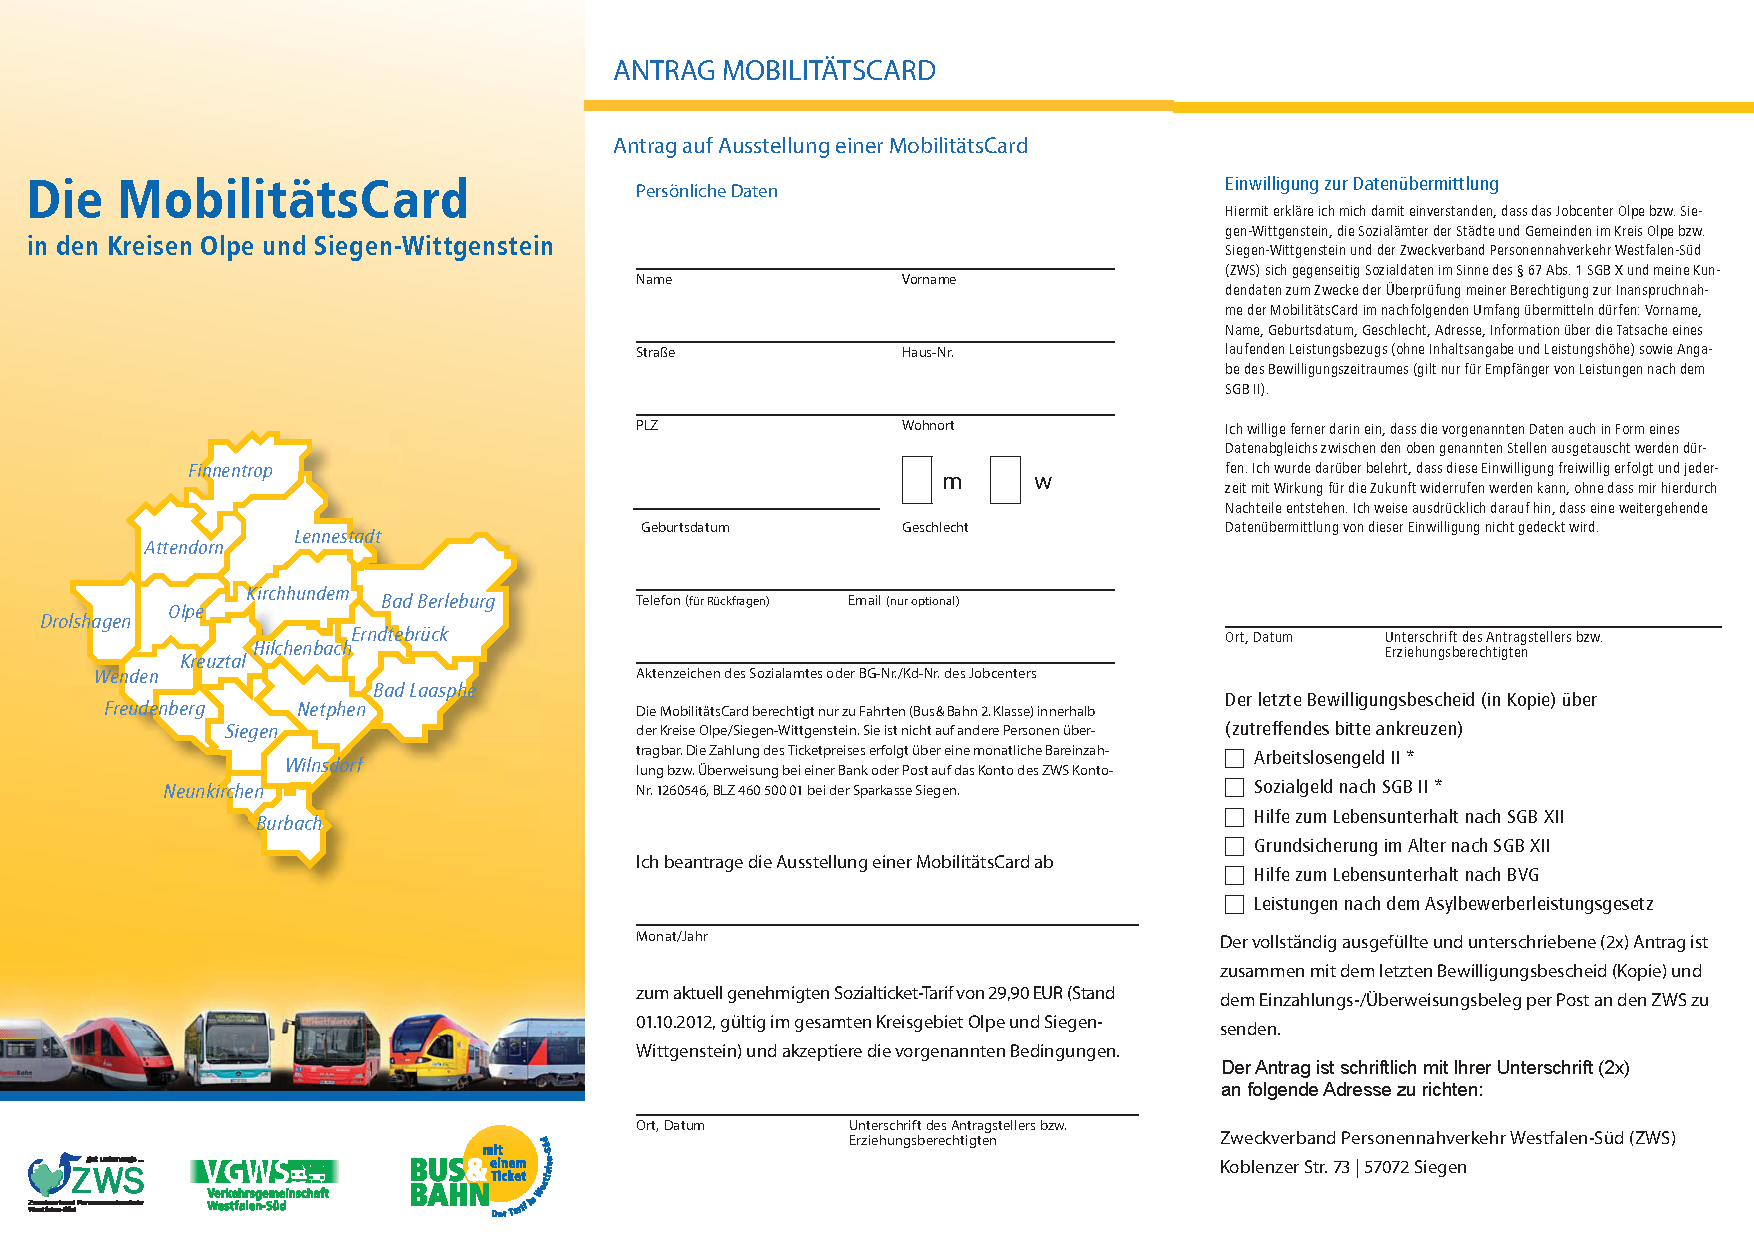
\includepdf[pages={-}]{quellen/1_MobilitaetsCard_Felder.pdf}
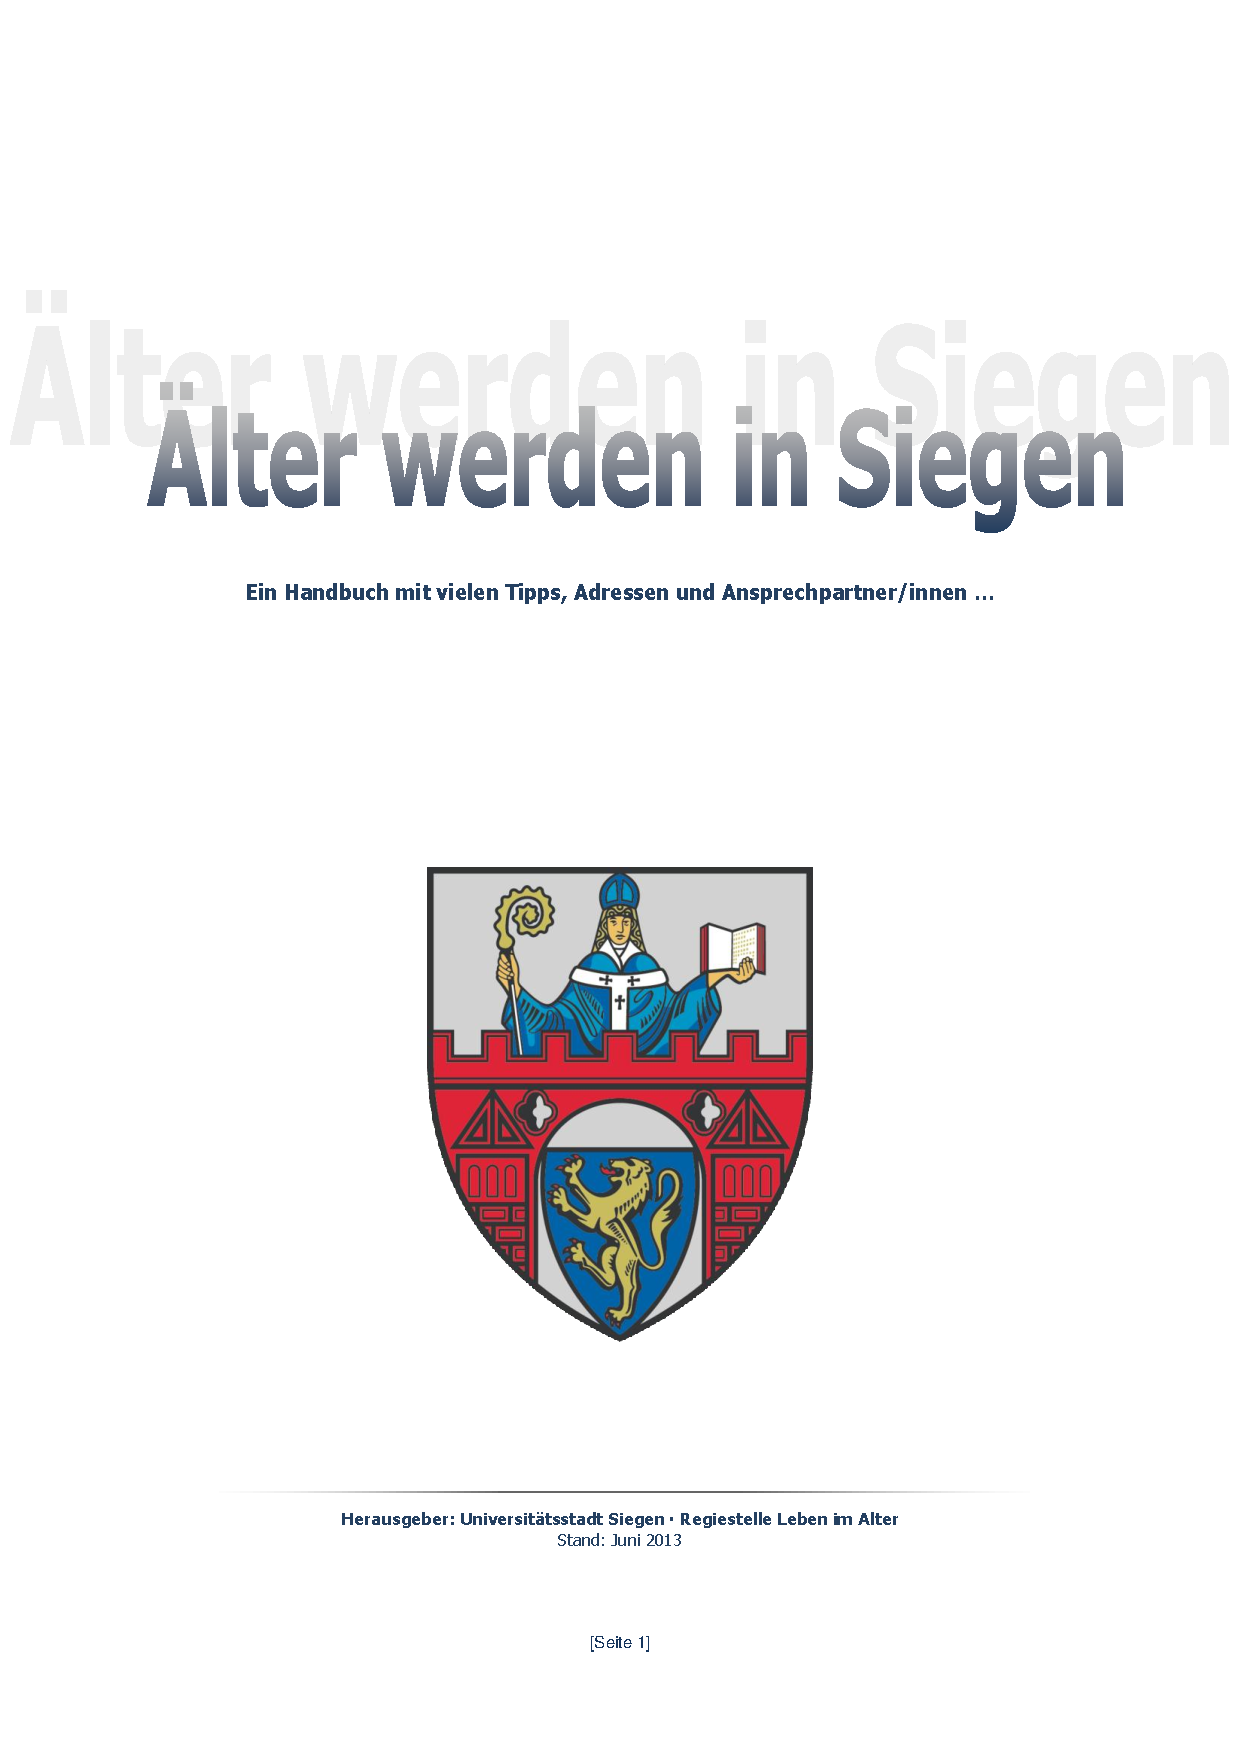
\includepdf[pages={-}]{quellen/HandbuchAelterWerdenInSiegenJuni2013.pdf}
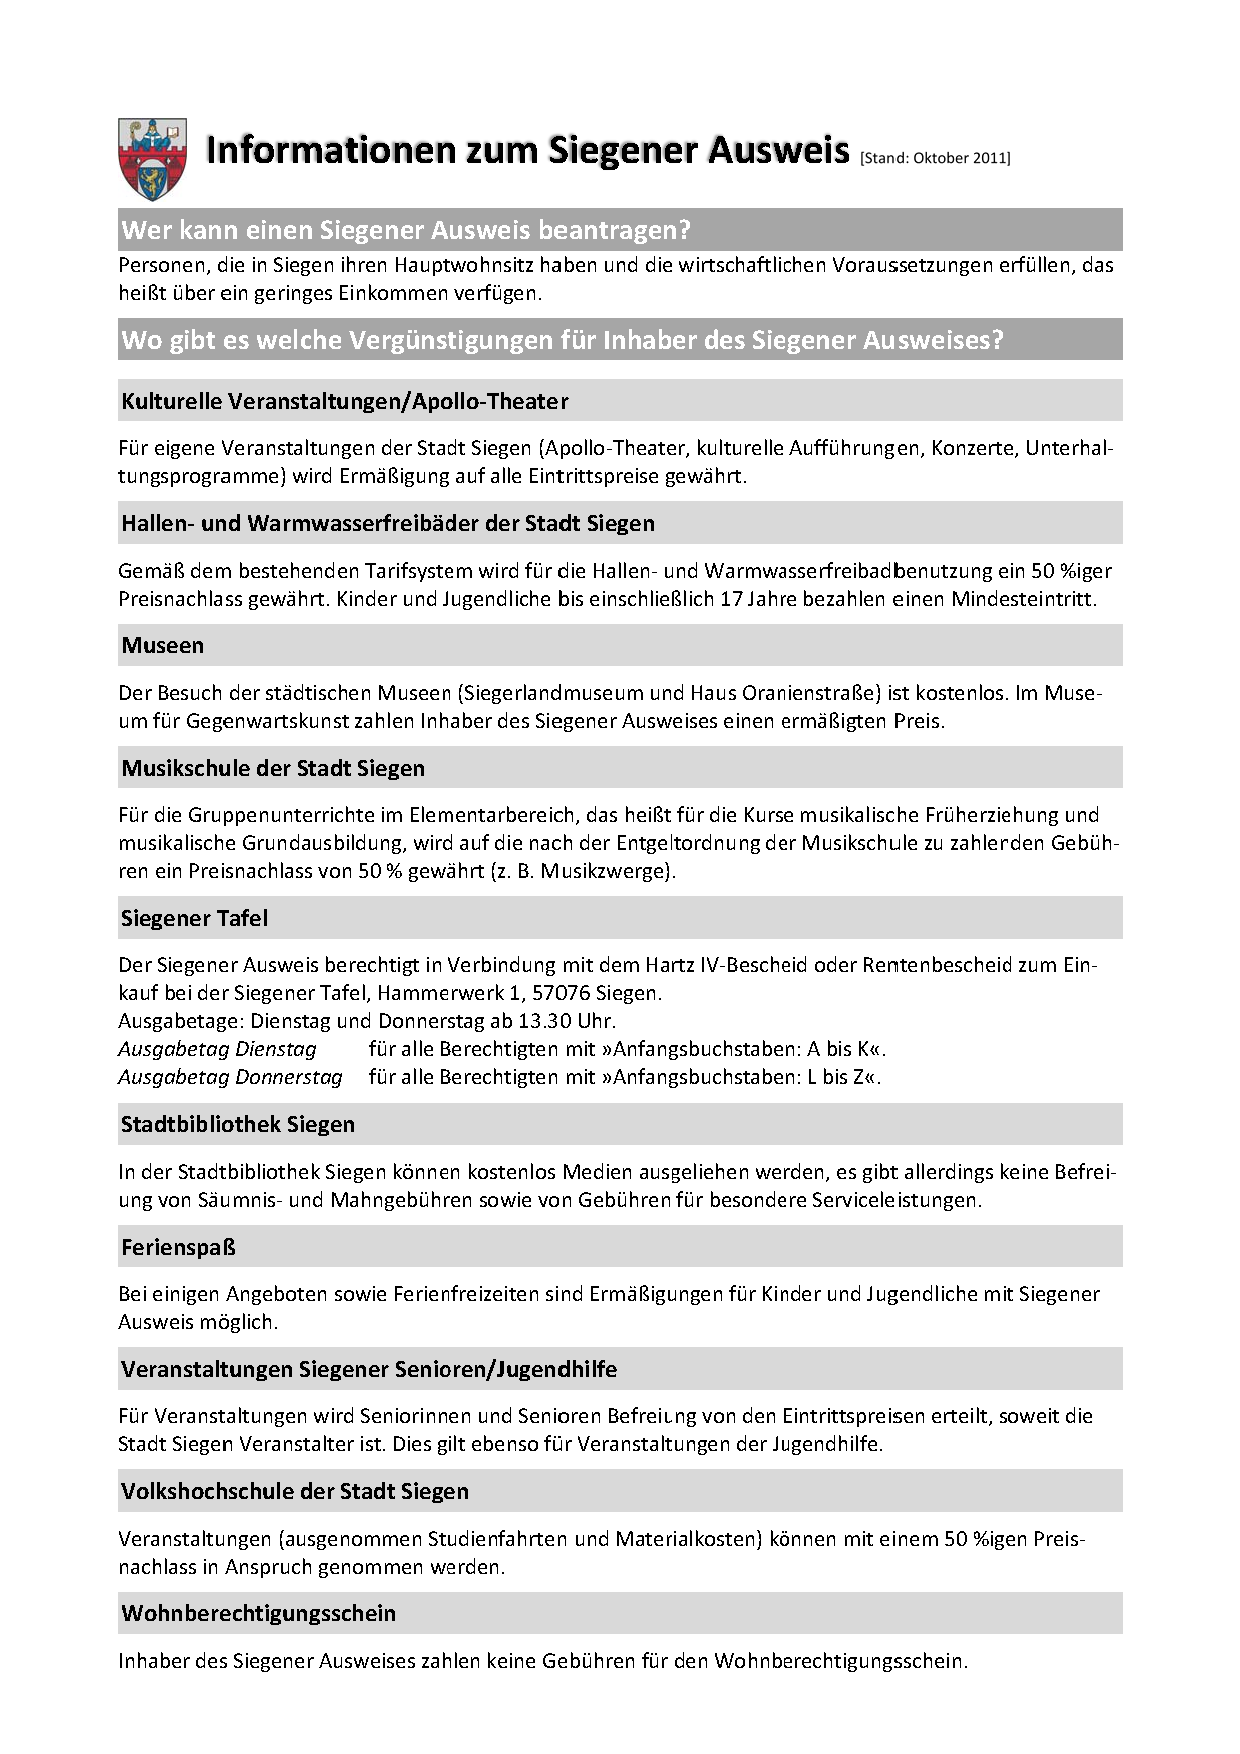
\includepdf[pages={-}]{quellen/Siegener_Ausweis_im_Internet_Oktober2011.pdf}



\end{document}